\documentclass[11pt]{article}
    \usepackage[breakable]{tcolorbox}
    \usepackage{parskip} % Stop auto-indenting (to mimic markdown behaviour)
    
    \usepackage{emoji}
    
    % Basic figure setup, for now with no caption control since it's done
    % automatically by Pandoc (which extracts ![](path) syntax from Markdown).
    \usepackage{graphicx}
    % Maintain compatibility with old templates. Remove in nbconvert 6.0
    \let\Oldincludegraphics\includegraphics
    % Ensure that by default, figures have no caption (until we provide a
    % proper Figure object with a Caption API and a way to capture that
    % in the conversion process - todo).
    \usepackage{caption}
    \DeclareCaptionFormat{nocaption}{}
    \captionsetup{format=nocaption,aboveskip=0pt,belowskip=0pt}

    \usepackage{float}
    \floatplacement{figure}{H} % forces figures to be placed at the correct location
    \usepackage{xcolor} % Allow colors to be defined
    \usepackage{enumerate} % Needed for markdown enumerations to work
    \usepackage{geometry} % Used to adjust the document margins
    \usepackage{amsmath} % Equations
    \usepackage{amssymb} % Equations
    \usepackage{textcomp} % defines textquotesingle
    % Hack from http://tex.stackexchange.com/a/47451/13684:
    \AtBeginDocument{%
        \def\PYZsq{\textquotesingle}% Upright quotes in Pygmentized code
    }
    \usepackage{upquote} % Upright quotes for verbatim code
    \usepackage{eurosym} % defines \euro

    \usepackage{iftex}
    \ifPDFTeX
        \usepackage[T1]{fontenc}
        \IfFileExists{alphabeta.sty}{
              \usepackage{alphabeta}
          }{
              \usepackage[mathletters]{ucs}
              \usepackage[utf8x]{inputenc}
          }
    \else
        \usepackage{fontspec}
        \usepackage{unicode-math}
    \fi

    \usepackage{fancyvrb} % verbatim replacement that allows latex
    \usepackage{grffile} % extends the file name processing of package graphics
                         % to support a larger range
    \makeatletter % fix for old versions of grffile with XeLaTeX
    \@ifpackagelater{grffile}{2019/11/01}
    {
      % Do nothing on new versions
    }
    {
      \def\Gread@@xetex#1{%
        \IfFileExists{"\Gin@base".bb}%
        {\Gread@eps{\Gin@base.bb}}%
        {\Gread@@xetex@aux#1}%
      }
    }
    \makeatother
    \usepackage[Export]{adjustbox} % Used to constrain images to a maximum size
    \adjustboxset{max size={0.9\linewidth}{0.9\paperheight}}

    % The hyperref package gives us a pdf with properly built
    % internal navigation ('pdf bookmarks' for the table of contents,
    % internal cross-reference links, web links for URLs, etc.)
    \usepackage{hyperref}
    % The default LaTeX title has an obnoxious amount of whitespace. By default,
    % titling removes some of it. It also provides customization options.
    \usepackage{titling}
    \usepackage{longtable} % longtable support required by pandoc >1.10
    \usepackage{booktabs}  % table support for pandoc > 1.12.2
    \usepackage{array}     % table support for pandoc >= 2.11.3
    \usepackage{calc}      % table minipage width calculation for pandoc >= 2.11.1
    \usepackage[inline]{enumitem} % IRkernel/repr support (it uses the enumerate* environment)
    \usepackage[normalem]{ulem} % ulem is needed to support strikethroughs (\sout)
                                % normalem makes italics be italics, not underlines
    \usepackage{mathrsfs}
    

    
    % Colors for the hyperref package
    \definecolor{urlcolor}{rgb}{0,.145,.698}
    \definecolor{linkcolor}{rgb}{.71,0.21,0.01}
    \definecolor{citecolor}{rgb}{.12,.54,.11}

    % ANSI colors
    \definecolor{ansi-black}{HTML}{3E424D}
    \definecolor{ansi-black-intense}{HTML}{282C36}
    \definecolor{ansi-red}{HTML}{E75C58}
    \definecolor{ansi-red-intense}{HTML}{B22B31}
    \definecolor{ansi-green}{HTML}{00A250}
    \definecolor{ansi-green-intense}{HTML}{007427}
    \definecolor{ansi-yellow}{HTML}{DDB62B}
    \definecolor{ansi-yellow-intense}{HTML}{B27D12}
    \definecolor{ansi-blue}{HTML}{208FFB}
    \definecolor{ansi-blue-intense}{HTML}{0065CA}
    \definecolor{ansi-magenta}{HTML}{D160C4}
    \definecolor{ansi-magenta-intense}{HTML}{A03196}
    \definecolor{ansi-cyan}{HTML}{60C6C8}
    \definecolor{ansi-cyan-intense}{HTML}{258F8F}
    \definecolor{ansi-white}{HTML}{C5C1B4}
    \definecolor{ansi-white-intense}{HTML}{A1A6B2}
    \definecolor{ansi-default-inverse-fg}{HTML}{FFFFFF}
    \definecolor{ansi-default-inverse-bg}{HTML}{000000}

    % common color for the border for error outputs.
    \definecolor{outerrorbackground}{HTML}{FFDFDF}

    % commands and environments needed by pandoc snippets
    % extracted from the output of `pandoc -s`
    \providecommand{\tightlist}{%
      \setlength{\itemsep}{0pt}\setlength{\parskip}{0pt}}
    \DefineVerbatimEnvironment{Highlighting}{Verbatim}{commandchars=\\\{\}}
    % Add ',fontsize=\small' for more characters per line
    \newenvironment{Shaded}{}{}
    \newcommand{\KeywordTok}[1]{\textcolor[rgb]{0.00,0.44,0.13}{\textbf{{#1}}}}
    \newcommand{\DataTypeTok}[1]{\textcolor[rgb]{0.56,0.13,0.00}{{#1}}}
    \newcommand{\DecValTok}[1]{\textcolor[rgb]{0.25,0.63,0.44}{{#1}}}
    \newcommand{\BaseNTok}[1]{\textcolor[rgb]{0.25,0.63,0.44}{{#1}}}
    \newcommand{\FloatTok}[1]{\textcolor[rgb]{0.25,0.63,0.44}{{#1}}}
    \newcommand{\CharTok}[1]{\textcolor[rgb]{0.25,0.44,0.63}{{#1}}}
    \newcommand{\StringTok}[1]{\textcolor[rgb]{0.25,0.44,0.63}{{#1}}}
    \newcommand{\CommentTok}[1]{\textcolor[rgb]{0.38,0.63,0.69}{\textit{{#1}}}}
    \newcommand{\OtherTok}[1]{\textcolor[rgb]{0.00,0.44,0.13}{{#1}}}
    \newcommand{\AlertTok}[1]{\textcolor[rgb]{1.00,0.00,0.00}{\textbf{{#1}}}}
    \newcommand{\FunctionTok}[1]{\textcolor[rgb]{0.02,0.16,0.49}{{#1}}}
    \newcommand{\RegionMarkerTok}[1]{{#1}}
    \newcommand{\ErrorTok}[1]{\textcolor[rgb]{1.00,0.00,0.00}{\textbf{{#1}}}}
    \newcommand{\NormalTok}[1]{{#1}}

    % Additional commands for more recent versions of Pandoc
    \newcommand{\ConstantTok}[1]{\textcolor[rgb]{0.53,0.00,0.00}{{#1}}}
    \newcommand{\SpecialCharTok}[1]{\textcolor[rgb]{0.25,0.44,0.63}{{#1}}}
    \newcommand{\VerbatimStringTok}[1]{\textcolor[rgb]{0.25,0.44,0.63}{{#1}}}
    \newcommand{\SpecialStringTok}[1]{\textcolor[rgb]{0.73,0.40,0.53}{{#1}}}
    \newcommand{\ImportTok}[1]{{#1}}
    \newcommand{\DocumentationTok}[1]{\textcolor[rgb]{0.73,0.13,0.13}{\textit{{#1}}}}
    \newcommand{\AnnotationTok}[1]{\textcolor[rgb]{0.38,0.63,0.69}{\textbf{\textit{{#1}}}}}
    \newcommand{\CommentVarTok}[1]{\textcolor[rgb]{0.38,0.63,0.69}{\textbf{\textit{{#1}}}}}
    \newcommand{\VariableTok}[1]{\textcolor[rgb]{0.10,0.09,0.49}{{#1}}}
    \newcommand{\ControlFlowTok}[1]{\textcolor[rgb]{0.00,0.44,0.13}{\textbf{{#1}}}}
    \newcommand{\OperatorTok}[1]{\textcolor[rgb]{0.40,0.40,0.40}{{#1}}}
    \newcommand{\BuiltInTok}[1]{{#1}}
    \newcommand{\ExtensionTok}[1]{{#1}}
    \newcommand{\PreprocessorTok}[1]{\textcolor[rgb]{0.74,0.48,0.00}{{#1}}}
    \newcommand{\AttributeTok}[1]{\textcolor[rgb]{0.49,0.56,0.16}{{#1}}}
    \newcommand{\InformationTok}[1]{\textcolor[rgb]{0.38,0.63,0.69}{\textbf{\textit{{#1}}}}}
    \newcommand{\WarningTok}[1]{\textcolor[rgb]{0.38,0.63,0.69}{\textbf{\textit{{#1}}}}}


    % Define a nice break command that doesn't care if a line doesn't already
    % exist.
    \def\br{\hspace*{\fill} \\* }
    % Math Jax compatibility definitions
    \def\gt{>}
    \def\lt{<}
    \let\Oldtex\TeX
    \let\Oldlatex\LaTeX
    \renewcommand{\TeX}{\textrm{\Oldtex}}
    \renewcommand{\LaTeX}{\textrm{\Oldlatex}}
    % Document parameters
    % Document title
    \title{Colored Camel}
    
    
    
    
    
% Pygments definitions
\makeatletter
\def\PY@reset{\let\PY@it=\relax \let\PY@bf=\relax%
    \let\PY@ul=\relax \let\PY@tc=\relax%
    \let\PY@bc=\relax \let\PY@ff=\relax}
\def\PY@tok#1{\csname PY@tok@#1\endcsname}
\def\PY@toks#1+{\ifx\relax#1\empty\else%
    \PY@tok{#1}\expandafter\PY@toks\fi}
\def\PY@do#1{\PY@bc{\PY@tc{\PY@ul{%
    \PY@it{\PY@bf{\PY@ff{#1}}}}}}}
\def\PY#1#2{\PY@reset\PY@toks#1+\relax+\PY@do{#2}}

\@namedef{PY@tok@w}{\def\PY@tc##1{\textcolor[rgb]{0.73,0.73,0.73}{##1}}}
\@namedef{PY@tok@c}{\let\PY@it=\textit\def\PY@tc##1{\textcolor[rgb]{0.24,0.48,0.48}{##1}}}
\@namedef{PY@tok@cp}{\def\PY@tc##1{\textcolor[rgb]{0.61,0.40,0.00}{##1}}}
\@namedef{PY@tok@k}{\let\PY@bf=\textbf\def\PY@tc##1{\textcolor[rgb]{0.00,0.50,0.00}{##1}}}
\@namedef{PY@tok@kp}{\def\PY@tc##1{\textcolor[rgb]{0.00,0.50,0.00}{##1}}}
\@namedef{PY@tok@kt}{\def\PY@tc##1{\textcolor[rgb]{0.69,0.00,0.25}{##1}}}
\@namedef{PY@tok@o}{\def\PY@tc##1{\textcolor[rgb]{0.40,0.40,0.40}{##1}}}
\@namedef{PY@tok@ow}{\let\PY@bf=\textbf\def\PY@tc##1{\textcolor[rgb]{0.67,0.13,1.00}{##1}}}
\@namedef{PY@tok@nb}{\def\PY@tc##1{\textcolor[rgb]{0.00,0.50,0.00}{##1}}}
\@namedef{PY@tok@nf}{\def\PY@tc##1{\textcolor[rgb]{0.00,0.00,1.00}{##1}}}
\@namedef{PY@tok@nc}{\let\PY@bf=\textbf\def\PY@tc##1{\textcolor[rgb]{0.00,0.00,1.00}{##1}}}
\@namedef{PY@tok@nn}{\let\PY@bf=\textbf\def\PY@tc##1{\textcolor[rgb]{0.00,0.00,1.00}{##1}}}
\@namedef{PY@tok@ne}{\let\PY@bf=\textbf\def\PY@tc##1{\textcolor[rgb]{0.80,0.25,0.22}{##1}}}
\@namedef{PY@tok@nv}{\def\PY@tc##1{\textcolor[rgb]{0.10,0.09,0.49}{##1}}}
\@namedef{PY@tok@no}{\def\PY@tc##1{\textcolor[rgb]{0.53,0.00,0.00}{##1}}}
\@namedef{PY@tok@nl}{\def\PY@tc##1{\textcolor[rgb]{0.46,0.46,0.00}{##1}}}
\@namedef{PY@tok@ni}{\let\PY@bf=\textbf\def\PY@tc##1{\textcolor[rgb]{0.44,0.44,0.44}{##1}}}
\@namedef{PY@tok@na}{\def\PY@tc##1{\textcolor[rgb]{0.41,0.47,0.13}{##1}}}
\@namedef{PY@tok@nt}{\let\PY@bf=\textbf\def\PY@tc##1{\textcolor[rgb]{0.00,0.50,0.00}{##1}}}
\@namedef{PY@tok@nd}{\def\PY@tc##1{\textcolor[rgb]{0.67,0.13,1.00}{##1}}}
\@namedef{PY@tok@s}{\def\PY@tc##1{\textcolor[rgb]{0.73,0.13,0.13}{##1}}}
\@namedef{PY@tok@sd}{\let\PY@it=\textit\def\PY@tc##1{\textcolor[rgb]{0.73,0.13,0.13}{##1}}}
\@namedef{PY@tok@si}{\let\PY@bf=\textbf\def\PY@tc##1{\textcolor[rgb]{0.64,0.35,0.47}{##1}}}
\@namedef{PY@tok@se}{\let\PY@bf=\textbf\def\PY@tc##1{\textcolor[rgb]{0.67,0.36,0.12}{##1}}}
\@namedef{PY@tok@sr}{\def\PY@tc##1{\textcolor[rgb]{0.64,0.35,0.47}{##1}}}
\@namedef{PY@tok@ss}{\def\PY@tc##1{\textcolor[rgb]{0.10,0.09,0.49}{##1}}}
\@namedef{PY@tok@sx}{\def\PY@tc##1{\textcolor[rgb]{0.00,0.50,0.00}{##1}}}
\@namedef{PY@tok@m}{\def\PY@tc##1{\textcolor[rgb]{0.40,0.40,0.40}{##1}}}
\@namedef{PY@tok@gh}{\let\PY@bf=\textbf\def\PY@tc##1{\textcolor[rgb]{0.00,0.00,0.50}{##1}}}
\@namedef{PY@tok@gu}{\let\PY@bf=\textbf\def\PY@tc##1{\textcolor[rgb]{0.50,0.00,0.50}{##1}}}
\@namedef{PY@tok@gd}{\def\PY@tc##1{\textcolor[rgb]{0.63,0.00,0.00}{##1}}}
\@namedef{PY@tok@gi}{\def\PY@tc##1{\textcolor[rgb]{0.00,0.52,0.00}{##1}}}
\@namedef{PY@tok@gr}{\def\PY@tc##1{\textcolor[rgb]{0.89,0.00,0.00}{##1}}}
\@namedef{PY@tok@ge}{\let\PY@it=\textit}
\@namedef{PY@tok@gs}{\let\PY@bf=\textbf}
\@namedef{PY@tok@gp}{\let\PY@bf=\textbf\def\PY@tc##1{\textcolor[rgb]{0.00,0.00,0.50}{##1}}}
\@namedef{PY@tok@go}{\def\PY@tc##1{\textcolor[rgb]{0.44,0.44,0.44}{##1}}}
\@namedef{PY@tok@gt}{\def\PY@tc##1{\textcolor[rgb]{0.00,0.27,0.87}{##1}}}
\@namedef{PY@tok@err}{\def\PY@bc##1{{\setlength{\fboxsep}{\string -\fboxrule}\fcolorbox[rgb]{1.00,0.00,0.00}{1,1,1}{\strut ##1}}}}
\@namedef{PY@tok@kc}{\let\PY@bf=\textbf\def\PY@tc##1{\textcolor[rgb]{0.00,0.50,0.00}{##1}}}
\@namedef{PY@tok@kd}{\let\PY@bf=\textbf\def\PY@tc##1{\textcolor[rgb]{0.00,0.50,0.00}{##1}}}
\@namedef{PY@tok@kn}{\let\PY@bf=\textbf\def\PY@tc##1{\textcolor[rgb]{0.00,0.50,0.00}{##1}}}
\@namedef{PY@tok@kr}{\let\PY@bf=\textbf\def\PY@tc##1{\textcolor[rgb]{0.00,0.50,0.00}{##1}}}
\@namedef{PY@tok@bp}{\def\PY@tc##1{\textcolor[rgb]{0.00,0.50,0.00}{##1}}}
\@namedef{PY@tok@fm}{\def\PY@tc##1{\textcolor[rgb]{0.00,0.00,1.00}{##1}}}
\@namedef{PY@tok@vc}{\def\PY@tc##1{\textcolor[rgb]{0.10,0.09,0.49}{##1}}}
\@namedef{PY@tok@vg}{\def\PY@tc##1{\textcolor[rgb]{0.10,0.09,0.49}{##1}}}
\@namedef{PY@tok@vi}{\def\PY@tc##1{\textcolor[rgb]{0.10,0.09,0.49}{##1}}}
\@namedef{PY@tok@vm}{\def\PY@tc##1{\textcolor[rgb]{0.10,0.09,0.49}{##1}}}
\@namedef{PY@tok@sa}{\def\PY@tc##1{\textcolor[rgb]{0.73,0.13,0.13}{##1}}}
\@namedef{PY@tok@sb}{\def\PY@tc##1{\textcolor[rgb]{0.73,0.13,0.13}{##1}}}
\@namedef{PY@tok@sc}{\def\PY@tc##1{\textcolor[rgb]{0.73,0.13,0.13}{##1}}}
\@namedef{PY@tok@dl}{\def\PY@tc##1{\textcolor[rgb]{0.73,0.13,0.13}{##1}}}
\@namedef{PY@tok@s2}{\def\PY@tc##1{\textcolor[rgb]{0.73,0.13,0.13}{##1}}}
\@namedef{PY@tok@sh}{\def\PY@tc##1{\textcolor[rgb]{0.73,0.13,0.13}{##1}}}
\@namedef{PY@tok@s1}{\def\PY@tc##1{\textcolor[rgb]{0.73,0.13,0.13}{##1}}}
\@namedef{PY@tok@mb}{\def\PY@tc##1{\textcolor[rgb]{0.40,0.40,0.40}{##1}}}
\@namedef{PY@tok@mf}{\def\PY@tc##1{\textcolor[rgb]{0.40,0.40,0.40}{##1}}}
\@namedef{PY@tok@mh}{\def\PY@tc##1{\textcolor[rgb]{0.40,0.40,0.40}{##1}}}
\@namedef{PY@tok@mi}{\def\PY@tc##1{\textcolor[rgb]{0.40,0.40,0.40}{##1}}}
\@namedef{PY@tok@il}{\def\PY@tc##1{\textcolor[rgb]{0.40,0.40,0.40}{##1}}}
\@namedef{PY@tok@mo}{\def\PY@tc##1{\textcolor[rgb]{0.40,0.40,0.40}{##1}}}
\@namedef{PY@tok@ch}{\let\PY@it=\textit\def\PY@tc##1{\textcolor[rgb]{0.24,0.48,0.48}{##1}}}
\@namedef{PY@tok@cm}{\let\PY@it=\textit\def\PY@tc##1{\textcolor[rgb]{0.24,0.48,0.48}{##1}}}
\@namedef{PY@tok@cpf}{\let\PY@it=\textit\def\PY@tc##1{\textcolor[rgb]{0.24,0.48,0.48}{##1}}}
\@namedef{PY@tok@c1}{\let\PY@it=\textit\def\PY@tc##1{\textcolor[rgb]{0.24,0.48,0.48}{##1}}}
\@namedef{PY@tok@cs}{\let\PY@it=\textit\def\PY@tc##1{\textcolor[rgb]{0.24,0.48,0.48}{##1}}}

\def\PYZbs{\char`\\}
\def\PYZus{\char`\_}
\def\PYZob{\char`\{}
\def\PYZcb{\char`\}}
\def\PYZca{\char`\^}
\def\PYZam{\char`\&}
\def\PYZlt{\char`\<}
\def\PYZgt{\char`\>}
\def\PYZsh{\char`\#}
\def\PYZpc{\char`\%}
\def\PYZdl{\char`\$}
\def\PYZhy{\char`\-}
\def\PYZsq{\char`\'}
\def\PYZdq{\char`\"}
\def\PYZti{\char`\~}
% for compatibility with earlier versions
\def\PYZat{@}
\def\PYZlb{[}
\def\PYZrb{]}
\makeatother


    % For linebreaks inside Verbatim environment from package fancyvrb.
    \makeatletter
        \newbox\Wrappedcontinuationbox
        \newbox\Wrappedvisiblespacebox
        \newcommand*\Wrappedvisiblespace {\textcolor{red}{\textvisiblespace}}
        \newcommand*\Wrappedcontinuationsymbol {\textcolor{red}{\llap{\tiny$\m@th\hookrightarrow$}}}
        \newcommand*\Wrappedcontinuationindent {3ex }
        \newcommand*\Wrappedafterbreak {\kern\Wrappedcontinuationindent\copy\Wrappedcontinuationbox}
        % Take advantage of the already applied Pygments mark-up to insert
        % potential linebreaks for TeX processing.
        %        {, <, #, %, $, ' and ": go to next line.
        %        _, }, ^, &, >, - and ~: stay at end of broken line.
        % Use of \textquotesingle for straight quote.
        \newcommand*\Wrappedbreaksatspecials {%
            \def\PYGZus{\discretionary{\char`\_}{\Wrappedafterbreak}{\char`\_}}%
            \def\PYGZob{\discretionary{}{\Wrappedafterbreak\char`\{}{\char`\{}}%
            \def\PYGZcb{\discretionary{\char`\}}{\Wrappedafterbreak}{\char`\}}}%
            \def\PYGZca{\discretionary{\char`\^}{\Wrappedafterbreak}{\char`\^}}%
            \def\PYGZam{\discretionary{\char`\&}{\Wrappedafterbreak}{\char`\&}}%
            \def\PYGZlt{\discretionary{}{\Wrappedafterbreak\char`\<}{\char`\<}}%
            \def\PYGZgt{\discretionary{\char`\>}{\Wrappedafterbreak}{\char`\>}}%
            \def\PYGZsh{\discretionary{}{\Wrappedafterbreak\char`\#}{\char`\#}}%
            \def\PYGZpc{\discretionary{}{\Wrappedafterbreak\char`\%}{\char`\%}}%
            \def\PYGZdl{\discretionary{}{\Wrappedafterbreak\char`\$}{\char`\$}}%
            \def\PYGZhy{\discretionary{\char`\-}{\Wrappedafterbreak}{\char`\-}}%
            \def\PYGZsq{\discretionary{}{\Wrappedafterbreak\textquotesingle}{\textquotesingle}}%
            \def\PYGZdq{\discretionary{}{\Wrappedafterbreak\char`\"}{\char`\"}}%
            \def\PYGZti{\discretionary{\char`\~}{\Wrappedafterbreak}{\char`\~}}%
        }
        % Some characters . , ; ? ! / are not pygmentized.
        % This macro makes them "active" and they will insert potential linebreaks
        \newcommand*\Wrappedbreaksatpunct {%
            \lccode`\~`\.\lowercase{\def~}{\discretionary{\hbox{\char`\.}}{\Wrappedafterbreak}{\hbox{\char`\.}}}%
            \lccode`\~`\,\lowercase{\def~}{\discretionary{\hbox{\char`\,}}{\Wrappedafterbreak}{\hbox{\char`\,}}}%
            \lccode`\~`\;\lowercase{\def~}{\discretionary{\hbox{\char`\;}}{\Wrappedafterbreak}{\hbox{\char`\;}}}%
            \lccode`\~`\:\lowercase{\def~}{\discretionary{\hbox{\char`\:}}{\Wrappedafterbreak}{\hbox{\char`\:}}}%
            \lccode`\~`\?\lowercase{\def~}{\discretionary{\hbox{\char`\?}}{\Wrappedafterbreak}{\hbox{\char`\?}}}%
            \lccode`\~`\!\lowercase{\def~}{\discretionary{\hbox{\char`\!}}{\Wrappedafterbreak}{\hbox{\char`\!}}}%
            \lccode`\~`\/\lowercase{\def~}{\discretionary{\hbox{\char`\/}}{\Wrappedafterbreak}{\hbox{\char`\/}}}%
            \catcode`\.\active
            \catcode`\,\active
            \catcode`\;\active
            \catcode`\:\active
            \catcode`\?\active
            \catcode`\!\active
            \catcode`\/\active
            \lccode`\~`\~
        }
    \makeatother

    \let\OriginalVerbatim=\Verbatim
    \makeatletter
    \renewcommand{\Verbatim}[1][1]{%
        %\parskip\z@skip
        \sbox\Wrappedcontinuationbox {\Wrappedcontinuationsymbol}%
        \sbox\Wrappedvisiblespacebox {\FV@SetupFont\Wrappedvisiblespace}%
        \def\FancyVerbFormatLine ##1{\hsize\linewidth
            \vtop{\raggedright\hyphenpenalty\z@\exhyphenpenalty\z@
                \doublehyphendemerits\z@\finalhyphendemerits\z@
                \strut ##1\strut}%
        }%
        % If the linebreak is at a space, the latter will be displayed as visible
        % space at end of first line, and a continuation symbol starts next line.
        % Stretch/shrink are however usually zero for typewriter font.
        \def\FV@Space {%
            \nobreak\hskip\z@ plus\fontdimen3\font minus\fontdimen4\font
            \discretionary{\copy\Wrappedvisiblespacebox}{\Wrappedafterbreak}
            {\kern\fontdimen2\font}%
        }%

        % Allow breaks at special characters using \PYG... macros.
        \Wrappedbreaksatspecials
        % Breaks at punctuation characters . , ; ? ! and / need catcode=\active
        \OriginalVerbatim[#1,codes*=\Wrappedbreaksatpunct]%
    }
    \makeatother

    % Exact colors from NB
    \definecolor{incolor}{HTML}{303F9F}
    \definecolor{outcolor}{HTML}{D84315}
    \definecolor{cellborder}{HTML}{CFCFCF}
    \definecolor{cellbackground}{HTML}{F7F7F7}

    % prompt
    \makeatletter
    \newcommand{\boxspacing}{\kern\kvtcb@left@rule\kern\kvtcb@boxsep}
    \makeatother
    \newcommand{\prompt}[4]{
        {\ttfamily\llap{{\color{#2}[#3]:\hspace{3pt}#4}}\vspace{-\baselineskip}}
    }
    

    
    % Prevent overflowing lines due to hard-to-break entities
    \sloppy
    % Setup hyperref package
    \hypersetup{
      breaklinks=true,  % so long urls are correctly broken across lines
      colorlinks=true,
      urlcolor=urlcolor,
      linkcolor=linkcolor,
      citecolor=citecolor,
      }
    % Slightly bigger margins than the latex defaults
    
    \geometry{verbose,tmargin=1in,bmargin=1in,lmargin=1in,rmargin=1in}
    
    

\begin{document}
    
    \begin{figure}
\centering

\includegraphics[width=\textwidth, keepaspectratio]{Colored Camel_files/logo.png}
\caption{logo.png}
\end{figure}
\tableofcontents

\newpage
\section{Algoritmo \& Progetto \emoji{orangutan}}
    \hypertarget{obiettivo}{%
\subsection{\texorpdfstring{Obiettivo }{Obiettivo }}\label{obiettivo}}

L'obiettivo di questo progetto è quello di realizzare un programma
scritto in \textbf{OCaml} che risolva il \emph{problema} della
\emph{colorazione di un grafo}: riuscire a colorare, se possibile, ogni
nodo del grafo in modo da non avere mai nodi adiacenti con lo stesso
colore. In via più formale, dato un grafo \(G\) ed un numero massimo di
colori utilizzabili \(N\), assegnare un colore (da \(0\) a \(N − 1\)) ai
nodi in modo tale che non esistano nodi adiacenti con lo stesso colore;
qualora il numero di colori \(N\) non sia sufficiente per realizzare la
colorazione, riportare un errore.

    \hypertarget{definizione-di-tipi-ed-eccezioni}{%
\subsection{\texorpdfstring{Definizione di Tipi ed Eccezioni
}{Definizione di Tipi ed Eccezioni }}\label{definizione-di-tipi-ed-eccezioni}}

    Definisco il tipo di dato \texttt{grafo} e \texttt{problema} con i
relativi costruttori di tipo \texttt{Grafo} e \texttt{Problema}. Il
primo tipo rappresenta un \emph{grafo}, quindi la funzione
\emph{successori} che dato un intero (un nodo) restituisce tutti i suoi
nodi vicini (i successori). Il secondo va a rappresentare il
\emph{problema da risolvere}, questo è composto da un \textbf{grafo}
(che andrà colorato), dal \textbf{nodo di partenza} e dal massimo numero
di \textbf{colori utilizzabili} \(N\).

    \begin{tcolorbox}[breakable, size=fbox, boxrule=1pt, pad at break*=1mm,colback=cellbackground, colframe=cellborder]
\prompt{In}{incolor}{1}{\boxspacing}
\begin{Verbatim}[commandchars=\\\{\}]
\PY{k}{type} \PY{n}{grafo} \PY{o}{=} \PY{n+nc}{Grafo} \PY{k}{of} \PY{o}{(}\PY{k+kt}{int} \PY{o}{\PYZhy{}\PYZgt{}} \PY{k+kt}{int} \PY{k+kt}{list}\PY{o}{)}\PY{o}{;;}
\PY{k}{type} \PY{n}{problema} \PY{o}{=} \PY{n+nc}{Problema} \PY{k}{of} \PY{n}{grafo} \PY{o}{*} \PY{k+kt}{int} \PY{o}{*} \PY{k+kt}{int}\PY{o}{;;}
\end{Verbatim}
\end{tcolorbox}
            \begin{tcolorbox}[breakable, size=fbox, boxrule=.5pt, pad at break*=1mm, opacityfill=0]
\prompt{Out}{outcolor}{1}{\boxspacing}
\begin{Verbatim}[commandchars=\\\{\}]
type grafo = Grafo of (int -> int list)
\end{Verbatim}
\prompt{Out}{outcolor}{1}{\boxspacing}
\begin{Verbatim}[commandchars=\\\{\}]
type problema = Problema of grafo * int * int

\end{Verbatim}
\end{tcolorbox}
        
    La seguente eccezione verrà lanciata per segnalare che il problema in
questione non è risolvibile dato che il grafo non è colorabile con il
numero di colori dato.

    \begin{tcolorbox}[breakable, size=fbox, boxrule=1pt, pad at break*=1mm,colback=cellbackground, colframe=cellborder]
\prompt{In}{incolor}{2}{\boxspacing}
\begin{Verbatim}[commandchars=\\\{\}]
\PY{k}{exception} \PY{n+nc}{NumeroColoriInsufficiente}\PY{o}{;;}
\end{Verbatim}
\end{tcolorbox}

            \begin{tcolorbox}[breakable, size=fbox, boxrule=.5pt, pad at break*=1mm, opacityfill=0]
\prompt{Out}{outcolor}{2}{\boxspacing}
\begin{Verbatim}[commandchars=\\\{\}]
exception NumeroColoriInsifficiente

\end{Verbatim}
\end{tcolorbox}

\newpage


\subsection{\texorpdfstring{Definizione dei Problemi
}{Definizione dei Problemi }}\label{definizione-dei-problemi}

    Ho deciso di rappresentare ogni grafo da colorare come un
\texttt{Problema} composto da 3 elementi distinti:

\begin{enumerate}
\def\labelenumi{\arabic{enumi}.}
\tightlist
\item
  \texttt{succ}: la funzione successori che definisce tutti i nodi
  vicini raggiungibili da ogni altro nodo. Questo rappresenta il
  \textbf{Grafo} da colorare
\item
  \texttt{start}: nodo di partenza per la colorazione
\item
  \texttt{maxColori}: numero massimo (\(N\)) di colori da utilizzare
  durante la colorazione
\end{enumerate}

    Per esempio, il problema costituito dal seguente grafo
    \begin{figure}[H]
        \centering
        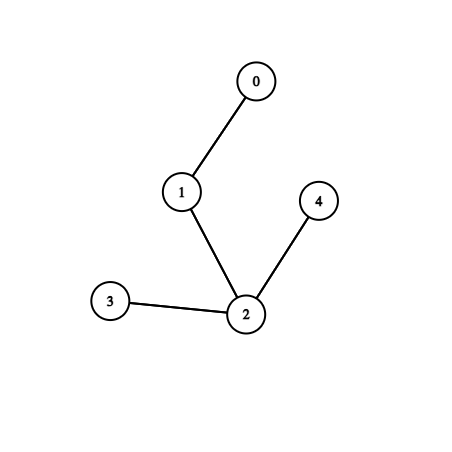
\includegraphics[width=8cm, keepaspectratio]{Colored Camel_files/graph7.png}
    \end{figure}
 con partenza dal nodo \(0\) e
con un numero di colori \(N=2\) è rappresentato dalla parte di codice
sottostante:

\begin{Shaded}
\begin{Highlighting}[]
\KeywordTok{let}\NormalTok{ problema =}
  \KeywordTok{let}\NormalTok{ x = }\KeywordTok{function}        
        \DecValTok{0}\NormalTok{ {-}\textgreater{} [}\DecValTok{1}\NormalTok{]}
\NormalTok{      | }\DecValTok{1}\NormalTok{ {-}\textgreater{} [}\DecValTok{0}\NormalTok{; }\DecValTok{2}\NormalTok{]}
\NormalTok{      | }\DecValTok{2}\NormalTok{ {-}\textgreater{} [}\DecValTok{1}\NormalTok{; }\DecValTok{3}\NormalTok{; }\DecValTok{4}\NormalTok{]}
\NormalTok{      | }\DecValTok{3}\NormalTok{ {-}\textgreater{} [}\DecValTok{2}\NormalTok{]}
\NormalTok{      | }\DecValTok{4}\NormalTok{ {-}\textgreater{} [}\DecValTok{2}\NormalTok{]}
\NormalTok{      | \_ {-}\textgreater{} [] }\KeywordTok{in}
  \KeywordTok{let}\NormalTok{ start = }\DecValTok{0} \KeywordTok{in}       \CommentTok{(* Partenza *)}
  \KeywordTok{let}\NormalTok{ maxColori = }\DecValTok{2} \KeywordTok{in}   \CommentTok{(* Massimo numero di colori*)}
  \KeywordTok{let} \DataTypeTok{succ}\NormalTok{ = Grafo x }\KeywordTok{in}  \CommentTok{(* Successori *)}

\NormalTok{  (Problema (}\DataTypeTok{succ}\NormalTok{, start, maxColori))}
\NormalTok{;;}
\end{Highlighting}
\end{Shaded}

    \hypertarget{problema-1}{%
\subsubsection{\texorpdfstring{Problema 1
}{Problema 1 }}\label{problema-1}}

    Il \textbf{problema 1} è formato da un grafo non orientato e sconnesso,
composto da 7 nodi. Il punto di partenza è il \emph{nodo 3} ed ha un
numero massimo di colori \(N = 3\). Questo problema è stato scelto per
far vedere come l'algoritmo si comporta con grafi sconnessi: andrà a
colorare solo i nodi che riesce a raggiungere.

    \begin{tcolorbox}[breakable, size=fbox, boxrule=1pt, pad at break*=1mm,colback=cellbackground, colframe=cellborder]
\prompt{In}{incolor}{3}{\boxspacing}
\begin{Verbatim}[commandchars=\\\{\}]
\PY{k}{let} \PY{n}{problema\PYZus{}1} \PY{o}{=}
  \PY{k}{let} \PY{n}{x} \PY{o}{=} \PY{k}{function}        
        \PY{l+m+mi}{0} \PY{o}{\PYZhy{}\PYZgt{}} \PY{o}{[}\PY{l+m+mi}{1}\PY{o}{;} \PY{l+m+mi}{2}\PY{o}{]}
      \PY{o}{|} \PY{l+m+mi}{1} \PY{o}{\PYZhy{}\PYZgt{}} \PY{o}{[}\PY{l+m+mi}{0}\PY{o}{;} \PY{l+m+mi}{2}\PY{o}{;} \PY{l+m+mi}{3}\PY{o}{]}
      \PY{o}{|} \PY{l+m+mi}{2} \PY{o}{\PYZhy{}\PYZgt{}} \PY{o}{[}\PY{l+m+mi}{0}\PY{o}{;} \PY{l+m+mi}{1}\PY{o}{]}
      \PY{o}{|} \PY{l+m+mi}{3} \PY{o}{\PYZhy{}\PYZgt{}} \PY{o}{[}\PY{l+m+mi}{1}\PY{o}{;} \PY{l+m+mi}{4}\PY{o}{]}
      \PY{o}{|} \PY{l+m+mi}{4} \PY{o}{\PYZhy{}\PYZgt{}} \PY{o}{[}\PY{l+m+mi}{3}\PY{o}{]}
      \PY{o}{|} \PY{l+m+mi}{5} \PY{o}{\PYZhy{}\PYZgt{}} \PY{o}{[}\PY{l+m+mi}{6}\PY{o}{]}
      \PY{o}{|} \PY{o}{\PYZus{}} \PY{o}{\PYZhy{}\PYZgt{}} \PY{n+nb+bp}{[]} \PY{k}{in}
  \PY{k}{let} \PY{n}{start} \PY{o}{=} \PY{l+m+mi}{3} \PY{k}{in}       \PY{c}{(*}\PY{c}{ Partenza }\PY{c}{*)}
  \PY{k}{let} \PY{n}{maxColori} \PY{o}{=} \PY{l+m+mi}{3} \PY{k}{in}   \PY{c}{(*}\PY{c}{ Massimo numero di colori}\PY{c}{*)}
  \PY{k}{let} \PY{n}{succ} \PY{o}{=} \PY{n+nc}{Grafo} \PY{n}{x} \PY{k}{in}  \PY{c}{(*}\PY{c}{ Successori }\PY{c}{*)}

  \PY{o}{(}\PY{n+nc}{Problema} \PY{o}{(}\PY{n}{succ}\PY{o}{,} \PY{n}{start}\PY{o}{,} \PY{n}{maxColori}\PY{o}{)}\PY{o}{)}
\PY{o}{;;}
\end{Verbatim}
\end{tcolorbox}

            \begin{tcolorbox}[breakable, size=fbox, boxrule=.5pt, pad at break*=1mm, opacityfill=0]
\prompt{Out}{outcolor}{3}{\boxspacing}
\begin{Verbatim}[commandchars=\\\{\}]
val problema\_1 : problema = Problema (Grafo <fun>, 3, 3)

\end{Verbatim}
\end{tcolorbox}
        
    \begin{figure}
\centering
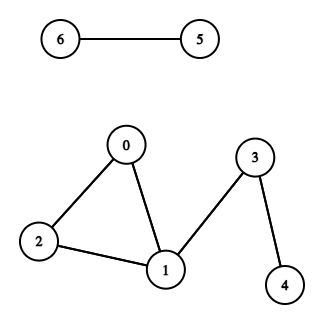
\includegraphics[width=7cm, keepaspectratio]{Colored Camel_files/graph1.png}
\caption{graph1.png}
\end{figure}

\newpage
    \hypertarget{problema-2}{%
\subsubsection{\texorpdfstring{Problema 2
}{Problema 2 }}\label{problema-2}}

    Questo problema è composto da un grafo non orientato e connesso che
presenta vari cicli. Ce ne sono 2 varianti:

\begin{enumerate}
\def\labelenumi{\arabic{enumi}.}
\tightlist
\item
  la prima è quella che può essere colorata senza problemi con partenza
  dal \emph{nodo 0} e numero massimo di colori \(N = 4\)
\item
  la seconda non è colorabile dato che il numero massimo di colori
  \(N = 3\) non risultano sufficienti per la risoluzione del problema
  (ne servono minimo 4).
\end{enumerate}

    \begin{tcolorbox}[breakable, size=fbox, boxrule=1pt, pad at break*=1mm,colback=cellbackground, colframe=cellborder]
\prompt{In}{incolor}{4}{\boxspacing}
\begin{Verbatim}[commandchars=\\\{\}]
\PY{k}{let} \PY{n}{problema\PYZus{}2\PYZus{}err} \PY{o}{=} 
  \PY{k}{let} \PY{n}{x} \PY{o}{=} \PY{k}{function}        
        \PY{l+m+mi}{0} \PY{o}{\PYZhy{}\PYZgt{}} \PY{o}{[}\PY{l+m+mi}{1}\PY{o}{;} \PY{l+m+mi}{2}\PY{o}{;} \PY{l+m+mi}{3}\PY{o}{;} \PY{l+m+mi}{4}\PY{o}{;} \PY{l+m+mi}{5}\PY{o}{]}
      \PY{o}{|} \PY{l+m+mi}{1} \PY{o}{\PYZhy{}\PYZgt{}} \PY{o}{[}\PY{l+m+mi}{0}\PY{o}{;} \PY{l+m+mi}{3}\PY{o}{]}
      \PY{o}{|} \PY{l+m+mi}{2} \PY{o}{\PYZhy{}\PYZgt{}} \PY{o}{[}\PY{l+m+mi}{0}\PY{o}{;} \PY{l+m+mi}{5}\PY{o}{;} \PY{l+m+mi}{4}\PY{o}{]}
      \PY{o}{|} \PY{l+m+mi}{3} \PY{o}{\PYZhy{}\PYZgt{}} \PY{o}{[}\PY{l+m+mi}{0}\PY{o}{;} \PY{l+m+mi}{1}\PY{o}{;} \PY{l+m+mi}{4}\PY{o}{]}
      \PY{o}{|} \PY{l+m+mi}{4} \PY{o}{\PYZhy{}\PYZgt{}} \PY{o}{[}\PY{l+m+mi}{0}\PY{o}{;} \PY{l+m+mi}{3}\PY{o}{;} \PY{l+m+mi}{2}\PY{o}{;} \PY{l+m+mi}{5}\PY{o}{]}
      \PY{o}{|} \PY{l+m+mi}{5} \PY{o}{\PYZhy{}\PYZgt{}} \PY{o}{[}\PY{l+m+mi}{0}\PY{o}{;} \PY{l+m+mi}{2}\PY{o}{;} \PY{l+m+mi}{4}\PY{o}{]}
      \PY{o}{|} \PY{o}{\PYZus{}} \PY{o}{\PYZhy{}\PYZgt{}} \PY{n+nb+bp}{[]} \PY{k}{in}

    \PY{k}{let} \PY{n}{start} \PY{o}{=} \PY{l+m+mi}{0} \PY{k}{in}       \PY{c}{(*}\PY{c}{ Partenza }\PY{c}{*)}
    \PY{k}{let} \PY{n}{maxColori} \PY{o}{=} \PY{l+m+mi}{3} \PY{k}{in}   \PY{c}{(*}\PY{c}{ Massimo numero di colori}\PY{c}{*)}
    \PY{k}{let} \PY{n}{succ} \PY{o}{=} \PY{n+nc}{Grafo} \PY{n}{x} \PY{k}{in}  \PY{c}{(*}\PY{c}{ Successori }\PY{c}{*)}
    
    \PY{o}{(}\PY{n+nc}{Problema} \PY{o}{(}\PY{n}{succ}\PY{o}{,} \PY{n}{start}\PY{o}{,} \PY{n}{maxColori}\PY{o}{)}\PY{o}{)}
\PY{o}{;;}
\end{Verbatim}
\end{tcolorbox}

            \begin{tcolorbox}[breakable, size=fbox, boxrule=.5pt, pad at break*=1mm, opacityfill=0]
\prompt{Out}{outcolor}{4}{\boxspacing}
\begin{Verbatim}[commandchars=\\\{\}]
val problema\_2\_err : problema = Problema (Grafo <fun>, 0, 3)

\end{Verbatim}
\end{tcolorbox}
        
    \begin{tcolorbox}[breakable, size=fbox, boxrule=1pt, pad at break*=1mm,colback=cellbackground, colframe=cellborder]
\prompt{In}{incolor}{5}{\boxspacing}
\begin{Verbatim}[commandchars=\\\{\}]
\PY{k}{let} \PY{n}{problema\PYZus{}2} \PY{o}{=} 
  \PY{k}{let} \PY{n}{x} \PY{o}{=} \PY{k}{function}        
        \PY{l+m+mi}{0} \PY{o}{\PYZhy{}\PYZgt{}} \PY{o}{[}\PY{l+m+mi}{1}\PY{o}{;} \PY{l+m+mi}{2}\PY{o}{;} \PY{l+m+mi}{3}\PY{o}{;} \PY{l+m+mi}{4}\PY{o}{;} \PY{l+m+mi}{5}\PY{o}{]}
      \PY{o}{|} \PY{l+m+mi}{1} \PY{o}{\PYZhy{}\PYZgt{}} \PY{o}{[}\PY{l+m+mi}{0}\PY{o}{;} \PY{l+m+mi}{3}\PY{o}{]}
      \PY{o}{|} \PY{l+m+mi}{2} \PY{o}{\PYZhy{}\PYZgt{}} \PY{o}{[}\PY{l+m+mi}{0}\PY{o}{;} \PY{l+m+mi}{5}\PY{o}{;} \PY{l+m+mi}{4}\PY{o}{]}
      \PY{o}{|} \PY{l+m+mi}{3} \PY{o}{\PYZhy{}\PYZgt{}} \PY{o}{[}\PY{l+m+mi}{0}\PY{o}{;} \PY{l+m+mi}{1}\PY{o}{;} \PY{l+m+mi}{4}\PY{o}{]}
      \PY{o}{|} \PY{l+m+mi}{4} \PY{o}{\PYZhy{}\PYZgt{}} \PY{o}{[}\PY{l+m+mi}{0}\PY{o}{;} \PY{l+m+mi}{3}\PY{o}{;} \PY{l+m+mi}{2}\PY{o}{;} \PY{l+m+mi}{5}\PY{o}{]}
      \PY{o}{|} \PY{l+m+mi}{5} \PY{o}{\PYZhy{}\PYZgt{}} \PY{o}{[}\PY{l+m+mi}{0}\PY{o}{;} \PY{l+m+mi}{2}\PY{o}{;} \PY{l+m+mi}{4}\PY{o}{]}
      \PY{o}{|} \PY{o}{\PYZus{}} \PY{o}{\PYZhy{}\PYZgt{}} \PY{n+nb+bp}{[]} \PY{k}{in}

    \PY{k}{let} \PY{n}{start} \PY{o}{=} \PY{l+m+mi}{0} \PY{k}{in}       \PY{c}{(*}\PY{c}{ Partenza }\PY{c}{*)}
    \PY{k}{let} \PY{n}{maxColori} \PY{o}{=} \PY{l+m+mi}{4} \PY{k}{in}   \PY{c}{(*}\PY{c}{ Massimo numero di colori}\PY{c}{*)}
    \PY{k}{let} \PY{n}{succ} \PY{o}{=} \PY{n+nc}{Grafo} \PY{n}{x} \PY{k}{in}  \PY{c}{(*}\PY{c}{ Successori }\PY{c}{*)}
    
    \PY{o}{(}\PY{n+nc}{Problema} \PY{o}{(}\PY{n}{succ}\PY{o}{,} \PY{n}{start}\PY{o}{,} \PY{n}{maxColori}\PY{o}{)}\PY{o}{)}
\PY{o}{;;}
\end{Verbatim}
\end{tcolorbox}

            \begin{tcolorbox}[breakable, size=fbox, boxrule=.5pt, pad at break*=1mm, opacityfill=0]
\prompt{Out}{outcolor}{5}{\boxspacing}
\begin{Verbatim}[commandchars=\\\{\}]
val problema\_2 : problema = Problema (Grafo <fun>, 0, 4)

\end{Verbatim}
\end{tcolorbox}
        
    \begin{figure}
\centering
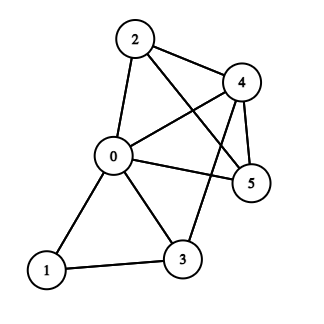
\includegraphics[width=8cm, keepaspectratio]{Colored Camel_files/graph2.png}
\caption{graph2.png}
\end{figure}

    \hypertarget{problema-3}{%
\subsubsection{\texorpdfstring{Problema 3
}{Problema 3 }}\label{problema-3}}

    Il \textbf{problema 3} ha un altro grafo con 7 nodi, con una topologia
abbastanza basilare, un numero massimo di colori \(N = 3\) ed il
\emph{nodo 0} come punto di partenza.

    \begin{tcolorbox}[breakable, size=fbox, boxrule=1pt, pad at break*=1mm,colback=cellbackground, colframe=cellborder]
\prompt{In}{incolor}{6}{\boxspacing}
\begin{Verbatim}[commandchars=\\\{\}]
\PY{k}{let} \PY{n}{problema\PYZus{}3} \PY{o}{=} 
  \PY{k}{let} \PY{n}{x} \PY{o}{=} \PY{k}{function}
      \PY{l+m+mi}{0} \PY{o}{\PYZhy{}\PYZgt{}} \PY{o}{[}\PY{l+m+mi}{1} \PY{o}{;} \PY{l+m+mi}{5}\PY{o}{]}
    \PY{o}{|} \PY{l+m+mi}{1} \PY{o}{\PYZhy{}\PYZgt{}} \PY{o}{[}\PY{l+m+mi}{0}\PY{o}{;} \PY{l+m+mi}{2}\PY{o}{]}
    \PY{o}{|} \PY{l+m+mi}{2} \PY{o}{\PYZhy{}\PYZgt{}} \PY{o}{[}\PY{l+m+mi}{5}\PY{o}{;} \PY{l+m+mi}{4}\PY{o}{;} \PY{l+m+mi}{3}\PY{o}{;} \PY{l+m+mi}{1}\PY{o}{;} \PY{l+m+mi}{6}\PY{o}{]}
    \PY{o}{|} \PY{l+m+mi}{3} \PY{o}{\PYZhy{}\PYZgt{}} \PY{o}{[}\PY{l+m+mi}{2}\PY{o}{;} \PY{l+m+mi}{6}\PY{o}{]}
    \PY{o}{|} \PY{l+m+mi}{4} \PY{o}{\PYZhy{}\PYZgt{}} \PY{o}{[}\PY{l+m+mi}{2}\PY{o}{]}
    \PY{o}{|} \PY{l+m+mi}{5} \PY{o}{\PYZhy{}\PYZgt{}} \PY{o}{[}\PY{l+m+mi}{0}\PY{o}{;} \PY{l+m+mi}{2}\PY{o}{]}
    \PY{o}{|} \PY{l+m+mi}{6} \PY{o}{\PYZhy{}\PYZgt{}} \PY{o}{[}\PY{l+m+mi}{2}\PY{o}{;} \PY{l+m+mi}{3}\PY{o}{]}
    \PY{o}{|} \PY{o}{\PYZus{}} \PY{o}{\PYZhy{}\PYZgt{}} \PY{n+nb+bp}{[]} \PY{k}{in}
    
    \PY{k}{let} \PY{n}{start} \PY{o}{=} \PY{l+m+mi}{0} \PY{k}{in}       \PY{c}{(*}\PY{c}{ Partenza }\PY{c}{*)}
    \PY{k}{let} \PY{n}{maxColori} \PY{o}{=} \PY{l+m+mi}{3} \PY{k}{in}   \PY{c}{(*}\PY{c}{ Massimo numero di colori}\PY{c}{*)}
    \PY{k}{let} \PY{n}{succ} \PY{o}{=} \PY{n+nc}{Grafo} \PY{n}{x} \PY{k}{in}  \PY{c}{(*}\PY{c}{ Successori }\PY{c}{*)}

    \PY{o}{(}\PY{n+nc}{Problema} \PY{o}{(}\PY{n}{succ}\PY{o}{,} \PY{n}{start}\PY{o}{,} \PY{n}{maxColori}\PY{o}{)}\PY{o}{)}
\PY{o}{;;}
\end{Verbatim}
\end{tcolorbox}

            \begin{tcolorbox}[breakable, size=fbox, boxrule=.5pt, pad at break*=1mm, opacityfill=0]
\prompt{Out}{outcolor}{6}{\boxspacing}
\begin{Verbatim}[commandchars=\\\{\}]
val problema\_3 : problema = Problema (Grafo <fun>, 0, 3)

\end{Verbatim}
\end{tcolorbox}
        
    \begin{figure}
\centering
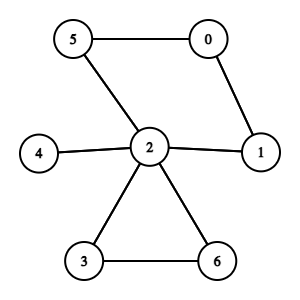
\includegraphics[width=7cm, keepaspectratio]{Colored Camel_files/graph3.png}
\caption{graph3.png}
\end{figure}

    \hypertarget{problema-4}{%
\subsubsection{\texorpdfstring{Problema 4
}{Problema 4 }}\label{problema-4}}

    Il grafo di questo problema è \emph{orientato} ed è stato scelto per
verificare il comportamento dell'algoritmo. Il \emph{nodo 0} è in
collegamento con tutti gli altri, ma questi non possono raggiungerlo. Il
punto di partenza è il \emph{nodo 0} ed ha un numero di colori massimo
\(N = 3\).

    \begin{tcolorbox}[breakable, size=fbox, boxrule=1pt, pad at break*=1mm,colback=cellbackground, colframe=cellborder]
\prompt{In}{incolor}{7}{\boxspacing}
\begin{Verbatim}[commandchars=\\\{\}]
\PY{k}{let} \PY{n}{problema\PYZus{}4} \PY{o}{=} 
  \PY{k}{let} \PY{n}{x} \PY{o}{=} \PY{k}{function}
      \PY{l+m+mi}{0} \PY{o}{\PYZhy{}\PYZgt{}} \PY{o}{[}\PY{l+m+mi}{1}\PY{o}{;} \PY{l+m+mi}{2}\PY{o}{;} \PY{l+m+mi}{3}\PY{o}{;} \PY{l+m+mi}{4}\PY{o}{]}
    \PY{o}{|} \PY{o}{\PYZus{}} \PY{o}{\PYZhy{}\PYZgt{}} \PY{n+nb+bp}{[]} \PY{k}{in}
    
    \PY{k}{let} \PY{n}{start} \PY{o}{=} \PY{l+m+mi}{0} \PY{k}{in}       \PY{c}{(*}\PY{c}{ Partenza }\PY{c}{*)}
    \PY{k}{let} \PY{n}{maxColori} \PY{o}{=} \PY{l+m+mi}{3} \PY{k}{in}   \PY{c}{(*}\PY{c}{ Massimo numero di colori}\PY{c}{*)}
    \PY{k}{let} \PY{n}{succ} \PY{o}{=} \PY{n+nc}{Grafo} \PY{n}{x} \PY{k}{in}  \PY{c}{(*}\PY{c}{ Successori }\PY{c}{*)}

    \PY{o}{(}\PY{n+nc}{Problema} \PY{o}{(}\PY{n}{succ}\PY{o}{,} \PY{n}{start}\PY{o}{,} \PY{n}{maxColori}\PY{o}{)}\PY{o}{)}
\PY{o}{;;}
\end{Verbatim}
\end{tcolorbox}

            \begin{tcolorbox}[breakable, size=fbox, boxrule=.5pt, pad at break*=1mm, opacityfill=0]
\prompt{Out}{outcolor}{7}{\boxspacing}
\begin{Verbatim}[commandchars=\\\{\}]
val problema\_4 : problema = Problema (Grafo <fun>, 0, 3)

\end{Verbatim}
\end{tcolorbox}
        
    \begin{figure}
\centering
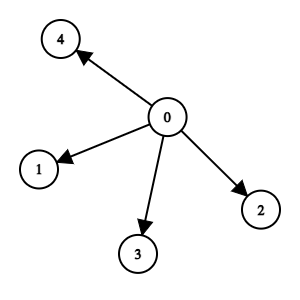
\includegraphics[width=7cm, keepaspectratio]{Colored Camel_files/graph4.png}
\caption{graph4.png}
\end{figure}

    \hypertarget{problema-5}{%
\subsubsection{\texorpdfstring{Problema 5
}{Problema 5 }}\label{problema-5}}

    Il grafo del \textbf{problema 5} ha un numero maggiore di nodi, con la
presenza di cicli e cammini ridondanti. È stato scelto per testare le
performance dell'algoritmo e per accertare la sua correttezza. Ha un
numero massimo di colori \(N = 2\) e come punto di partenza il
\emph{nodo 0}.

    \begin{tcolorbox}[breakable, size=fbox, boxrule=1pt, pad at break*=1mm,colback=cellbackground, colframe=cellborder]
\prompt{In}{incolor}{8}{\boxspacing}
\begin{Verbatim}[commandchars=\\\{\}]
\PY{k}{let} \PY{n}{problema\PYZus{}5} \PY{o}{=} 
  \PY{k}{let} \PY{n}{x} \PY{o}{=} \PY{k}{function}
       \PY{l+m+mi}{0} \PY{o}{\PYZhy{}\PYZgt{}} \PY{o}{[}\PY{l+m+mi}{1}\PY{o}{;} \PY{l+m+mi}{2}\PY{o}{;} \PY{l+m+mi}{6}\PY{o}{;} \PY{l+m+mi}{7}\PY{o}{]}
    \PY{o}{|}  \PY{l+m+mi}{1} \PY{o}{\PYZhy{}\PYZgt{}} \PY{o}{[}\PY{l+m+mi}{0}\PY{o}{;} \PY{l+m+mi}{8}\PY{o}{]}
    \PY{o}{|}  \PY{l+m+mi}{2} \PY{o}{\PYZhy{}\PYZgt{}} \PY{o}{[}\PY{l+m+mi}{0}\PY{o}{;} \PY{l+m+mi}{3}\PY{o}{]}
    \PY{o}{|}  \PY{l+m+mi}{3} \PY{o}{\PYZhy{}\PYZgt{}} \PY{o}{[}\PY{l+m+mi}{2}\PY{o}{;}\PY{l+m+mi}{4}\PY{o}{;}\PY{l+m+mi}{5}\PY{o}{]}
    \PY{o}{|}  \PY{l+m+mi}{4} \PY{o}{\PYZhy{}\PYZgt{}} \PY{o}{[}\PY{l+m+mi}{3}\PY{o}{;}\PY{l+m+mi}{5}\PY{o}{]}
    \PY{o}{|}  \PY{l+m+mi}{5} \PY{o}{\PYZhy{}\PYZgt{}} \PY{o}{[}\PY{l+m+mi}{3}\PY{o}{;}\PY{l+m+mi}{4}\PY{o}{;}\PY{l+m+mi}{6}\PY{o}{;}\PY{l+m+mi}{10}\PY{o}{]}
    \PY{o}{|}  \PY{l+m+mi}{6} \PY{o}{\PYZhy{}\PYZgt{}} \PY{o}{[}\PY{l+m+mi}{0}\PY{o}{;}\PY{l+m+mi}{5}\PY{o}{]}
    \PY{o}{|}  \PY{l+m+mi}{7} \PY{o}{\PYZhy{}\PYZgt{}} \PY{o}{[}\PY{l+m+mi}{0}\PY{o}{;}\PY{l+m+mi}{8}\PY{o}{]}
    \PY{o}{|}  \PY{l+m+mi}{8} \PY{o}{\PYZhy{}\PYZgt{}} \PY{o}{[}\PY{l+m+mi}{1}\PY{o}{;}\PY{l+m+mi}{7}\PY{o}{]}
    \PY{o}{|} \PY{l+m+mi}{10} \PY{o}{\PYZhy{}\PYZgt{}} \PY{o}{[}\PY{l+m+mi}{5}\PY{o}{]}
    \PY{o}{|} \PY{o}{\PYZus{}}  \PY{o}{\PYZhy{}\PYZgt{}} \PY{n+nb+bp}{[]} \PY{k}{in}
    
    \PY{k}{let} \PY{n}{start} \PY{o}{=} \PY{l+m+mi}{0} \PY{k}{in}       \PY{c}{(*}\PY{c}{ Partenza }\PY{c}{*)}
    \PY{k}{let} \PY{n}{maxColori} \PY{o}{=} \PY{l+m+mi}{2} \PY{k}{in}   \PY{c}{(*}\PY{c}{ Massimo numero di colori}\PY{c}{*)}
    \PY{k}{let} \PY{n}{succ} \PY{o}{=} \PY{n+nc}{Grafo} \PY{n}{x} \PY{k}{in}  \PY{c}{(*}\PY{c}{ Successori }\PY{c}{*)}

    \PY{o}{(}\PY{n+nc}{Problema} \PY{o}{(}\PY{n}{succ}\PY{o}{,} \PY{n}{start}\PY{o}{,} \PY{n}{maxColori}\PY{o}{)}\PY{o}{)}
\PY{o}{;;}
\end{Verbatim}
\end{tcolorbox}

            \begin{tcolorbox}[breakable, size=fbox, boxrule=.5pt, pad at break*=1mm, opacityfill=0]
\prompt{Out}{outcolor}{8}{\boxspacing}
\begin{Verbatim}[commandchars=\\\{\}]
val problema\_5 : problema = Problema (Grafo <fun>, 0, 2)

\end{Verbatim}
\end{tcolorbox}
        
    \begin{figure}
\centering
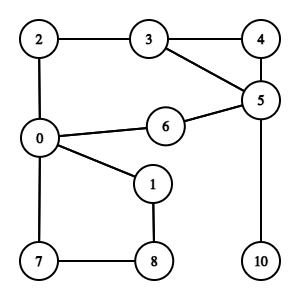
\includegraphics[width=6cm, keepaspectratio]{Colored Camel_files/graph5.png}
\caption{graph5.png}
\end{figure}

    \hypertarget{problema-6}{%
\subsubsection{\texorpdfstring{Problema 6
}{Problema 6 }}\label{problema-6}}

    L'ultimo problema è formato da un grafo abbastanza grande, con un
elevato numero di nodi, presenza di cicli e cammini ridondanti. Anche
questo è stato utilizzato per vedere come si comporta l'algoritmo su
grafi di modeste dimensioni.

    \begin{tcolorbox}[breakable, size=fbox, boxrule=1pt, pad at break*=1mm,colback=cellbackground, colframe=cellborder]
\prompt{In}{incolor}{9}{\boxspacing}
\begin{Verbatim}[commandchars=\\\{\}]
\PY{k}{let} \PY{n}{problema\PYZus{}6} \PY{o}{=} 
  \PY{k}{let} \PY{n}{x} \PY{o}{=} \PY{k}{function}
       \PY{l+m+mi}{0} \PY{o}{\PYZhy{}\PYZgt{}} \PY{o}{[}\PY{l+m+mi}{1}\PY{o}{]}
    \PY{o}{|}  \PY{l+m+mi}{1} \PY{o}{\PYZhy{}\PYZgt{}} \PY{o}{[}\PY{l+m+mi}{0}\PY{o}{;} \PY{l+m+mi}{2}\PY{o}{;} \PY{l+m+mi}{3}\PY{o}{]}
    \PY{o}{|}  \PY{l+m+mi}{2} \PY{o}{\PYZhy{}\PYZgt{}} \PY{o}{[}\PY{l+m+mi}{1}\PY{o}{;} \PY{l+m+mi}{4}\PY{o}{;} \PY{l+m+mi}{5}\PY{o}{]}
    \PY{o}{|}  \PY{l+m+mi}{3} \PY{o}{\PYZhy{}\PYZgt{}} \PY{o}{[}\PY{l+m+mi}{1}\PY{o}{;} \PY{l+m+mi}{12}\PY{o}{]}
    \PY{o}{|}  \PY{l+m+mi}{4} \PY{o}{\PYZhy{}\PYZgt{}} \PY{o}{[}\PY{l+m+mi}{2}\PY{o}{;} \PY{l+m+mi}{6}\PY{o}{]}
    \PY{o}{|}  \PY{l+m+mi}{5} \PY{o}{\PYZhy{}\PYZgt{}} \PY{o}{[}\PY{l+m+mi}{2}\PY{o}{;} \PY{l+m+mi}{11}\PY{o}{]}
    \PY{o}{|}  \PY{l+m+mi}{6} \PY{o}{\PYZhy{}\PYZgt{}} \PY{o}{[}\PY{l+m+mi}{4}\PY{o}{;} \PY{l+m+mi}{7}\PY{o}{;} \PY{l+m+mi}{8}\PY{o}{]}
    \PY{o}{|}  \PY{l+m+mi}{7} \PY{o}{\PYZhy{}\PYZgt{}} \PY{o}{[}\PY{l+m+mi}{6}\PY{o}{;} \PY{l+m+mi}{10}\PY{o}{]}
    \PY{o}{|}  \PY{l+m+mi}{8} \PY{o}{\PYZhy{}\PYZgt{}} \PY{o}{[}\PY{l+m+mi}{6}\PY{o}{;} \PY{l+m+mi}{9}\PY{o}{;} \PY{l+m+mi}{10}\PY{o}{]}
    \PY{o}{|}  \PY{l+m+mi}{9} \PY{o}{\PYZhy{}\PYZgt{}} \PY{o}{[}\PY{l+m+mi}{8}\PY{o}{;} \PY{l+m+mi}{11}\PY{o}{]}
    \PY{o}{|} \PY{l+m+mi}{10} \PY{o}{\PYZhy{}\PYZgt{}} \PY{o}{[}\PY{l+m+mi}{7}\PY{o}{;} \PY{l+m+mi}{12}\PY{o}{;} \PY{l+m+mi}{13}\PY{o}{]}
    \PY{o}{|} \PY{l+m+mi}{11} \PY{o}{\PYZhy{}\PYZgt{}} \PY{o}{[}\PY{l+m+mi}{5}\PY{o}{;} \PY{l+m+mi}{9}\PY{o}{;} \PY{l+m+mi}{15}\PY{o}{]}
    \PY{o}{|} \PY{l+m+mi}{12} \PY{o}{\PYZhy{}\PYZgt{}} \PY{o}{[}\PY{l+m+mi}{3}\PY{o}{;} \PY{l+m+mi}{10}\PY{o}{;} \PY{l+m+mi}{13}\PY{o}{]}
    \PY{o}{|} \PY{l+m+mi}{13} \PY{o}{\PYZhy{}\PYZgt{}} \PY{o}{[}\PY{l+m+mi}{10}\PY{o}{;} \PY{l+m+mi}{12}\PY{o}{;} \PY{l+m+mi}{14}\PY{o}{;} \PY{l+m+mi}{16}\PY{o}{]}
    \PY{o}{|} \PY{l+m+mi}{14} \PY{o}{\PYZhy{}\PYZgt{}} \PY{o}{[}\PY{l+m+mi}{13}\PY{o}{]}
    \PY{o}{|} \PY{l+m+mi}{15} \PY{o}{\PYZhy{}\PYZgt{}} \PY{o}{[}\PY{l+m+mi}{11}\PY{o}{]}
    \PY{o}{|} \PY{l+m+mi}{16} \PY{o}{\PYZhy{}\PYZgt{}} \PY{o}{[}\PY{l+m+mi}{13}\PY{o}{;} \PY{l+m+mi}{17}\PY{o}{]}
    \PY{o}{|} \PY{l+m+mi}{17} \PY{o}{\PYZhy{}\PYZgt{}} \PY{o}{[}\PY{l+m+mi}{16}\PY{o}{]}
    \PY{o}{|} \PY{o}{\PYZus{}}  \PY{o}{\PYZhy{}\PYZgt{}} \PY{n+nb+bp}{[]} \PY{k}{in}
  \PY{k}{let} \PY{n}{start} \PY{o}{=} \PY{l+m+mi}{0} \PY{k}{in}       \PY{c}{(*}\PY{c}{ Partenza }\PY{c}{*)}
  \PY{k}{let} \PY{n}{maxColori} \PY{o}{=} \PY{l+m+mi}{3} \PY{k}{in}   \PY{c}{(*}\PY{c}{ Massimo numero di colori}\PY{c}{*)}
  \PY{k}{let} \PY{n}{succ} \PY{o}{=} \PY{n+nc}{Grafo} \PY{n}{x} \PY{k}{in}  \PY{c}{(*}\PY{c}{ Successori }\PY{c}{*)}
  \PY{o}{(}\PY{n+nc}{Problema} \PY{o}{(}\PY{n}{succ}\PY{o}{,} \PY{n}{start}\PY{o}{,} \PY{n}{maxColori}\PY{o}{)}\PY{o}{)}
\PY{o}{;;}
\end{Verbatim}
\end{tcolorbox}

            \begin{tcolorbox}[breakable, size=fbox, boxrule=.5pt, pad at break*=1mm, opacityfill=0]
\prompt{Out}{outcolor}{9}{\boxspacing}
\begin{Verbatim}[commandchars=\\\{\}]
val problema\_6 : problema = Problema (Grafo <fun>, 0, 3)
\end{Verbatim}
\end{tcolorbox}
        
    \begin{figure}
\centering
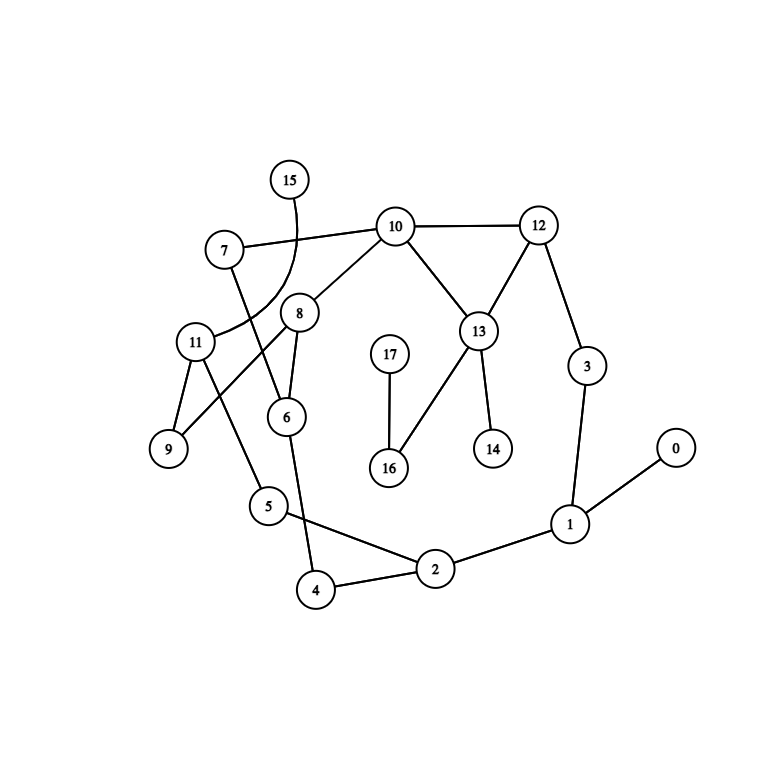
\includegraphics[width=15cm, keepaspectratio]{Colored Camel_files/graph6-2.png}
\caption{graph6-2.png}
\end{figure}

    \hypertarget{inclusione-moduli} e \texttt{\%\%}) sono solo disponibili con il
kernel python \emoji{pensive-face}.

    \begin{tcolorbox}[breakable, size=fbox, boxrule=1pt, pad at break*=1mm,colback=cellbackground, colframe=cellborder]
\prompt{In}{incolor}{10}{\boxspacing}
\begin{Verbatim}[commandchars=\\\{\}]
\PY{o}{\PYZsh{}}\PY{n}{require} \PY{l+s+s2}{\PYZdq{}}\PY{l+s+s2}{jupyter.notebook}\PY{l+s+s2}{\PYZdq{}} \PY{o}{;;}
\PY{k}{open} \PY{n+nc}{Jupyter\PYZus{}notebook} \PY{o}{;;}
\end{Verbatim}
\end{tcolorbox}

    \hypertarget{librerie-python}{%
\subsection{\texorpdfstring{Librerie Python
}{Librerie Python }}\label{librerie-python}}

    Procedo all'installazione (tramite \texttt{pip}) delle librerie
necessarie al funzionamento dello script python.

    \begin{tcolorbox}[breakable, size=fbox, boxrule=1pt, pad at break*=1mm,colback=cellbackground, colframe=cellborder]
\prompt{In}{incolor}{11}{\boxspacing}
\begin{Verbatim}[commandchars=\\\{\}]
\PY{n+nn}{Process}\PY{p}{.}\PY{n}{sh} \PY{l+s+s2}{\PYZdq{}}\PY{l+s+s2}{pip3 install matplotlib}\PY{l+s+s2}{\PYZdq{}}\PY{o}{;;}
\PY{n+nn}{Process}\PY{p}{.}\PY{n}{sh} \PY{l+s+s2}{\PYZdq{}}\PY{l+s+s2}{pip3 install pyvis}\PY{l+s+s2}{\PYZdq{}}\PY{o}{;;}
\end{Verbatim}
\end{tcolorbox}

    
        
    \hypertarget{idea-dellalgoritmo}{%
\subsection{\texorpdfstring{Idea dell'Algoritmo
}{Idea dell'Algoritmo }}\label{idea-dellalgoritmo}}

    L'idea su cui si basa questo algoritmo è quella di andare ad aggiornare
i colori dei vicini di un nodo se questi hanno lo stesso colore.

Prima di iniziare la fase di colorazione viene inizializzata una lista
con elementi formati da coppie \texttt{(nodo,\ colore)}. Questa
rappresenterà il risultato finale ed inizialmente tutti i nodi avranno
colore \texttt{0}. Viene creata esplorando il grafo (tramite una BFS)
iniziando dal nodo di partenza e, se siamo di fronte ad un grafo
sconnesso verrà presa in considerazione solo la parte di nodi
raggiungibile dal quello iniziale ignorando così gli altri.

Ora avviene la fase di colorazione dove, si parte dal nodo iniziale e,
sempre con una BFS, si va a scandire il grafo effettuando queste
operazioni:

\begin{itemize}
\tightlist
\item
  Controllo che il nodo che sto esaminando non sia già stato visitato,
  nel caso lo ignoro e proseguo con il prossimo
\item
  Per ogni suo vicino, controllo che il colore del vicino ed il suo
  siano uguali, se lo sono incremento di 1 il colore del vicino,
  altrimenti lascio tutto inalterato.
\item
  Prima di effettuare l'aggiornamento del colore di un nodo controllo di
  non aver superato il massimo numero di colori \(N\):

  \begin{itemize}
  \tightlist
  \item
    se ciò accade, arresto l'esecuzione e avviso l'utente che il
    problema non è risolvibile,
  \item
    altrimenti procedo con l'assegnamento e l'esplorazione
  \end{itemize}
\item
  Continuo fin quando non ho esplorato tutto il grafo.
\end{itemize}

    \hypertarget{funzioni-ausiliarie}{%
\subsection{\texorpdfstring{Funzioni Ausiliarie
}{Funzioni Ausiliarie }}\label{funzioni-ausiliarie}}

    Ritorna il colore del \texttt{nodo} dato. La funzione va a cercare il
nodo all'interno della lista di nodi colorati (risultato) e ritorna il
suo colore. La lista \texttt{colorati} è composta da coppie del tipo
\texttt{(nodo,\ colore).}

    \begin{tcolorbox}[breakable, size=fbox, boxrule=1pt, pad at break*=1mm,colback=cellbackground, colframe=cellborder]
\prompt{In}{incolor}{11}{\boxspacing}
\begin{Verbatim}[commandchars=\\\{\}]
\PY{k}{let} \PY{n}{get\PYZus{}colore} \PY{n}{nodo} \PY{n}{colorati} \PY{o}{=} 
  \PY{k}{let} \PY{k}{rec} \PY{n}{aux} \PY{n}{nodo} \PY{o}{=} \PY{k}{function} \PY{c}{(*}\PY{c}{lista di nodi colorati}\PY{c}{*)}
      \PY{o}{(}\PY{n}{x}\PY{o}{,}\PY{n}{y}\PY{o}{)}\PY{o}{::}\PY{n}{coda} \PY{o}{\PYZhy{}\PYZgt{}}    \PY{c}{(*}\PY{c}{prende il primo elemento della forma }\PY{c}{(}\PY{c}{x,y}\PY{c}{)}\PY{c}{*)}
        \PY{k}{if} \PY{n}{x} \PY{o}{=} \PY{n}{nodo}     \PY{c}{(*}\PY{c}{  se l\PYZsq{}elemento in questione è il nodo che cerco}\PY{c}{*)}
          \PY{k}{then} \PY{n}{y}        \PY{c}{(*}\PY{c}{    ritorna il colore del nodo}\PY{c}{*)}
        \PY{k}{else} 
          \PY{n}{aux} \PY{n}{nodo} \PY{n}{coda} \PY{c}{(*}\PY{c}{  continua con la ricorsione}\PY{c}{*)}

      \PY{o}{|} \PY{o}{\PYZus{}} \PY{o}{\PYZhy{}\PYZgt{}} \PY{o}{(}\PY{o}{\PYZhy{}}\PY{l+m+mi}{1}\PY{o}{)}  \PY{c}{(*}\PY{c}{se la lista finisce vuol dire che il nodo non esiste.}\PY{c}{*)}

  \PY{k}{in} \PY{n}{aux} \PY{n}{nodo} \PY{n}{colorati}   
  \PY{c}{(*}\PY{c}{avvia la ricorsione cone nodo=nodo lista\PYZus{}di\PYZus{}nodi\PYZus{}colorati=colorati}\PY{c}{*)}
\PY{o}{;;}
\end{Verbatim}
\end{tcolorbox}

            \begin{tcolorbox}[breakable, size=fbox, boxrule=.5pt, pad at break*=1mm, opacityfill=0]
\prompt{Out}{outcolor}{11}{\boxspacing}
\begin{Verbatim}[commandchars=\\\{\}]
val get\_colore : 'a -> ('a * int) list -> int = <fun>

\end{Verbatim}
\end{tcolorbox}

\newpage
        
Aggiorna i colori dei nodi adiacenti a quello in esame. Modifica la
lista \texttt{risultato} incrementando (\texttt{colore\ +\ 1}) il colore
dei nodi vicini a quello preso in esame solo se hanno lo stesso colore.
Quando si cerca di assegnare un nuovo colore si controlla prima che non
venga superato il limite massimo di colori utilizzabili, se succede,
viene lanciata un'eccezione e termina il programma.

    \begin{tcolorbox}[breakable, size=fbox, boxrule=1pt, pad at break*=1mm,colback=cellbackground, colframe=cellborder]
\prompt{In}{incolor}{12}{\boxspacing}
\begin{Verbatim}[commandchars=\\\{\}]
\PY{k}{let} \PY{n}{incrementa\PYZus{}colore\PYZus{}nodi} \PY{n}{risultato} \PY{n}{nodi} \PY{n}{colore} \PY{n}{maxColori} \PY{o}{=} 
  \PY{n+nn}{List}\PY{p}{.}\PY{n}{map} \PY{o}{(}
      \PY{k}{fun}\PY{o}{(}\PY{n}{x}\PY{o}{,} \PY{n}{y}\PY{o}{)} \PY{o}{\PYZhy{}\PYZgt{}} 
                \PY{c}{(*}\PY{c}{prende solo i        controlla che il colore            }\PY{c}{*)}
                \PY{c}{(*}\PY{c}{nodi vicini          del vicino sia uguale a quello del }\PY{c}{*)}
                \PY{c}{(*}\PY{c}{al nodo dato         nodo in esame                      }\PY{c}{*)}
          \PY{k}{if} \PY{o}{(}\PY{o}{(}\PY{n+nn}{List}\PY{p}{.}\PY{n}{mem} \PY{n}{x} \PY{n}{nodi}\PY{o}{)} \PY{o}{\PYZam{}\PYZam{}} \PY{o}{(}\PY{n}{colore}\PY{o}{=}\PY{o}{(}\PY{n}{get\PYZus{}colore} \PY{n}{x} \PY{n}{risultato}\PY{o}{)}\PY{o}{)}\PY{o}{)} 
              \PY{k}{then} 
                  \PY{k}{let} \PY{n}{nuovo\PYZus{}colore} \PY{o}{=} \PY{n}{y} \PY{o}{+} \PY{l+m+mi}{1} \PY{k}{in}
                  \PY{k}{if} \PY{o}{(}\PY{o}{(}\PY{n}{nuovo\PYZus{}colore}\PY{o}{)} \PY{o}{\PYZgt{}}\PY{o}{=} \PY{n}{maxColori}\PY{o}{)}        
                  \PY{c}{(*}\PY{c}{coltrolla che il numero massimo di colori}\PY{c}{*)}
                  \PY{c}{(*}\PY{c}{non venga superato                       }\PY{c}{*)}
                      \PY{k}{then}                               
                          \PY{k}{raise} \PY{n+nc}{NumeroColoriInsufficiente}
                  \PY{k}{else} 
                      \PY{o}{(}\PY{n}{x}\PY{o}{,} \PY{n}{nuovo\PYZus{}colore}\PY{o}{)}
          \PY{k}{else} 
              \PY{o}{(}\PY{n}{x}\PY{o}{,} \PY{n}{y}\PY{o}{)}
      \PY{o}{)} \PY{n}{risultato}
\PY{o}{;;}
\end{Verbatim}
\end{tcolorbox}

            \begin{tcolorbox}[breakable, size=fbox, boxrule=.5pt, pad at break*=1mm, opacityfill=0]
\prompt{Out}{outcolor}{12}{\boxspacing}
\begin{Verbatim}[commandchars=\\\{\}]
val incrementa\_colore\_nodi :
  ('a * int) list -> 'a list -> int -> int -> ('a * int) list = <fun>

\end{Verbatim}
\end{tcolorbox}
        
    Questa funzione crea una lista formata da coppie del tipo
\texttt{(nodo,\ colore)}. Questa lista rappresenta il risultato finale
della colorazione ed inizialmente viene assegnato ad ogni nodo il colore
\texttt{0}, che poi verrà modificato in seguito durante la risoluzione
del problema. Questa lista viene creata esplorando il grafo del problema
tramite una BFS.

    \begin{tcolorbox}[breakable, size=fbox, boxrule=1pt, pad at break*=1mm,colback=cellbackground, colframe=cellborder]
\prompt{In}{incolor}{13}{\boxspacing}
\begin{Verbatim}[commandchars=\\\{\}]
\PY{k}{let} \PY{n}{inizializza\PYZus{}risultato} \PY{o}{(}\PY{n+nc}{Grafo} \PY{n}{succ}\PY{o}{)} \PY{n}{partenza} \PY{o}{=}
  \PY{k}{let} \PY{k}{rec} \PY{n}{bfs} \PY{n}{visitati} \PY{n}{risultato} \PY{o}{=} \PY{k}{function} \PY{c}{(*}\PY{c}{ frontiera }\PY{c}{*)}
      \PY{n+nb+bp}{[]} \PY{o}{\PYZhy{}\PYZgt{}} \PY{n}{risultato}   \PY{c}{(*}\PY{c}{esplorazione finita, ritorno il risultato}\PY{c}{*)}
    \PY{o}{|} \PY{n}{nodo}\PY{o}{::}\PY{n}{coda} \PY{o}{\PYZhy{}\PYZgt{}}
      \PY{k}{if} \PY{n+nn}{List}\PY{p}{.}\PY{n}{mem} \PY{n}{nodo} \PY{n}{visitati}           \PY{c}{(*}\PY{c}{se il nodo è gia stato visitato}\PY{c}{*)}
        \PY{k}{then} 
          \PY{n}{bfs} \PY{n}{visitati} \PY{n}{risultato} \PY{n}{coda} \PY{c}{(*}\PY{c}{lo ignoro e continuo l\PYZsq{}esplorazione}\PY{c}{*)}
      \PY{k}{else}
        \PY{n}{bfs}                               \PY{c}{(*}\PY{c}{procedo con l\PYZsq{}esplorazione}\PY{c}{*)}
          \PY{o}{(}\PY{n}{visitati}\PY{o}{@}\PY{o}{[}\PY{n}{nodo}\PY{o}{]}\PY{o}{)}
          \PY{c}{(*}\PY{c}{aggiungo il nodo attuale alla frontiera}\PY{c}{*)}
          \PY{o}{(}\PY{n}{risultato}\PY{o}{@}\PY{o}{[}\PY{o}{(}\PY{n}{nodo}\PY{o}{,} \PY{l+m+mi}{0}\PY{o}{)}\PY{o}{]}\PY{o}{)}  
          \PY{c}{(*}\PY{c}{assegno il colore iniziale al nodo attuale}\PY{c}{*)}
          \PY{o}{(}\PY{n}{coda}\PY{o}{@}\PY{o}{(}\PY{n}{succ} \PY{n}{nodo}\PY{o}{)}\PY{o}{)}
          \PY{c}{(*}\PY{c}{aggiungo alla coda di nodi da esaminare i vicini del nodo attuale}\PY{c}{*)}

      \PY{k}{in} \PY{n}{bfs} \PY{n+nb+bp}{[]} \PY{n+nb+bp}{[]} \PY{o}{[}\PY{n}{partenza}\PY{o}{]}
    \PY{o}{;;}
\end{Verbatim}
\end{tcolorbox}

            \begin{tcolorbox}[breakable, size=fbox, boxrule=.5pt, pad at break*=1mm, opacityfill=0]
\prompt{Out}{outcolor}{13}{\boxspacing}
\begin{Verbatim}[commandchars=\\\{\}]
val inizializza\_risultato : grafo -> int -> (int * int) list = <fun>

\end{Verbatim}
\end{tcolorbox}
        
    Genera un file contenente il risultato della colorazione che verrà
passato a python per poter visualizzare il grafo in un modo più
comprensibile.

    \begin{tcolorbox}[breakable, size=fbox, boxrule=1pt, pad at break*=1mm,colback=cellbackground, colframe=cellborder]
\prompt{In}{incolor}{14}{\boxspacing}
\begin{Verbatim}[commandchars=\\\{\}]
\PY{k}{let} \PY{n}{grafodati\PYZus{}file} \PY{o}{=} \PY{l+s+s2}{\PYZdq{}}\PY{l+s+s2}{grafo.data}\PY{l+s+s2}{\PYZdq{}}\PY{o}{;;} \PY{c}{(*}\PY{c}{file su cui viene salvato il grafo}\PY{c}{*)}
\PY{k}{let} \PY{n}{salva\PYZus{}grafo\PYZus{}colorato} \PY{o}{(}\PY{n+nc}{Grafo} \PY{n}{succ}\PY{o}{)} \PY{n}{colorati} \PY{o}{=} 
  \PY{k}{let} \PY{n}{oc} \PY{o}{=} \PY{n}{open\PYZus{}out} \PY{n}{grafodati\PYZus{}file} \PY{k}{in}  \PY{c}{(*}\PY{c}{Apertura del file in scrittura}\PY{c}{*)}
    \PY{k}{let} \PY{k}{rec} \PY{n}{salva\PYZus{}lista} \PY{o}{=} 
    \PY{c}{(*}\PY{c}{Funzione ausiliaria per salvare su file una lista data}\PY{c}{*)}
      \PY{k}{function} \PY{c}{(*}\PY{c}{ lista }\PY{c}{*)}
         \PY{o}{[}\PY{n}{x}\PY{o}{]}      \PY{o}{\PYZhy{}\PYZgt{}} \PY{n+nn}{Printf}\PY{p}{.}\PY{n}{fprintf} \PY{n}{oc} \PY{l+s+s2}{\PYZdq{}}\PY{l+s+s2}{\PYZpc{}d}\PY{l+s+s2}{\PYZdq{}} \PY{n}{x}   
         \PY{c}{(*}\PY{c}{ caso base, se la lista ha un solo elemento lo stampa }\PY{c}{(}\PY{c}{senza \PYZdq{} \PYZdq{}}\PY{c}{)}\PY{c}{*)}
        \PY{o}{|} \PY{n}{x}\PY{o}{::}\PY{n}{coda} \PY{o}{\PYZhy{}\PYZgt{}}                            
        \PY{c}{(*}\PY{c}{ caso ricorsivo, la lista ha più elementi}\PY{c}{*)}            
          \PY{n+nn}{Printf}\PY{p}{.}\PY{n}{fprintf} \PY{n}{oc} \PY{l+s+s2}{\PYZdq{}}\PY{l+s+s2}{\PYZpc{}d }\PY{l+s+s2}{\PYZdq{}} \PY{n}{x}\PY{o}{;}            \PY{c}{(*}\PY{c}{  stampa l\PYZsq{}elemento}\PY{c}{*)}
          \PY{n}{salva\PYZus{}lista} \PY{n}{coda}                      \PY{c}{(*}\PY{c}{  continua la ricorsione}\PY{c}{*)}
        \PY{o}{|} \PY{o}{\PYZus{}} \PY{o}{\PYZhy{}\PYZgt{}} \PY{n+nb+bp}{()}
    \PY{k}{in} \PY{k}{let} \PY{k}{rec} \PY{n}{salva} \PY{o}{=}                                
    \PY{c}{(*}\PY{c}{Funzione ausiliaria per salvare nodo \PYZhy{} vicini \PYZhy{} colore su file}\PY{c}{*)}
      \PY{k}{function} \PY{c}{(*}\PY{c}{ lista nodi\PYZus{}colorati }\PY{c}{*)}
         \PY{n+nb+bp}{[]} \PY{o}{\PYZhy{}\PYZgt{}} \PY{n+nn}{Printf}\PY{p}{.}\PY{n}{fprintf} \PY{n}{oc} \PY{l+s+s2}{\PYZdq{}}\PY{l+s+se}{\PYZbs{}n}\PY{l+s+s2}{\PYZdq{}}\PY{o}{;} \PY{n}{close\PYZus{}out} \PY{n}{oc}   
         \PY{c}{(*}\PY{c}{ caso base, la lista è finita. Stampo un \PYZbs{}n e chiudo il file}\PY{c}{*)}
        \PY{o}{|}\PY{o}{(}\PY{n}{nodo}\PY{o}{,} \PY{n}{colore}\PY{o}{)}\PY{o}{::}\PY{n}{coda} \PY{o}{\PYZhy{}\PYZgt{}}                      
        \PY{c}{(*}\PY{c}{ caso ricorsivo, stampo nodo,lista vicini,colore nodo}\PY{c}{*)}
          \PY{n+nn}{Printf}\PY{p}{.}\PY{n}{fprintf} \PY{n}{oc} \PY{l+s+s2}{\PYZdq{}}\PY{l+s+s2}{\PYZpc{}d,}\PY{l+s+s2}{\PYZdq{}} \PY{n}{nodo}\PY{o}{;} \PY{n}{salva\PYZus{}lista} \PY{o}{(}\PY{n}{succ} \PY{n}{nodo}\PY{o}{)}\PY{o}{;} \PY{n+nn}{Printf}\PY{p}{.}\PY{n}{fprintf} \PY{n}{oc} \PY{l+s+s2}{\PYZdq{}}\PY{l+s+s2}{,}\PY{l+s+s2}{\PYZdq{}}\PY{o}{;} \PY{n+nn}{Printf}\PY{p}{.}\PY{n}{fprintf} \PY{n}{oc} \PY{l+s+s2}{\PYZdq{}}\PY{l+s+s2}{\PYZpc{}d}\PY{l+s+se}{\PYZbs{}n}\PY{l+s+s2}{\PYZdq{}} \PY{n}{colore}\PY{o}{;} 
          \PY{n}{salva} \PY{n}{coda}

    \PY{k}{in} \PY{n}{salva} \PY{n}{colorati} 
    \PY{c}{(*}\PY{c}{avvia la funzione ausiliaria per salvare il grafo su file}\PY{c}{*)}
\PY{o}{;;}
\end{Verbatim}
\end{tcolorbox}

        
            \begin{tcolorbox}[breakable, size=fbox, boxrule=.5pt, pad at break*=1mm, opacityfill=0]
\prompt{Out}{outcolor}{14}{\boxspacing}
\begin{Verbatim}[commandchars=\\\{\}]
val salva\_grafo\_colorato : grafo -> (int * int) list -> unit = <fun>

\end{Verbatim}
\end{tcolorbox}
        
Il successivo set di funzioni serve per mostrare immagini all'interno del
notebook ed avviare lo script in python responsabile della
rappresentazione grafica del risultato della colorazione. È anche
presente una funzione per la rimozione dei file temporanei, come il
risultato della risoluzione del problema che OCaml passerà a python o
l'immagine generata dallo script. La funzione \texttt{rappresenta} è
quella che combina tutte le altre per ottenere il risultato desiderato e
questa verrà invocata solo quando la colorazione del grafo sarà completa
ed avvenuta con successo.

Nelle varie funzioni ausiliare c'è una parte di codice comune a tutte,
\texttt{forza\_unit}, definita come segue:

\begin{Shaded}
\begin{Highlighting}[]
\KeywordTok{let}\NormalTok{ forza\_unit \_ = ();;}
\end{Highlighting}
\end{Shaded}

Questo permette di ignorare il valore di ritorno di qualunque
espressione passata a questa funzione ed ottenere così \texttt{unit}
come valore finale di ogni espressione.

    \begin{tcolorbox}[breakable, size=fbox, boxrule=1pt, pad at break*=1mm,colback=cellbackground, colframe=cellborder]
\prompt{In}{incolor}{15}{\boxspacing}
\begin{Verbatim}[commandchars=\\\{\}]
\PY{c}{(*}\PY{c}{forza unit come valore di ritorno ignorando quello dell\PYZsq{}espressione data}\PY{c}{*)}
\PY{k}{let} \PY{n}{forza\PYZus{}unit} \PY{o}{\PYZus{}} \PY{o}{=} \PY{n+nb+bp}{()}\PY{o}{;;}       
\PY{k}{let} \PY{n}{avvia\PYZus{}python} \PY{o}{=} \PY{k}{fun} \PY{n+nb+bp}{()} \PY{o}{\PYZhy{}\PYZgt{}}
    \PY{n}{forza\PYZus{}unit} \PY{o}{(}\PY{n+nn}{Process}\PY{p}{.}\PY{n}{sh} \PY{l+s+s2}{\PYZdq{}}\PY{l+s+s2}{python3 progetto/src/rappresentazione\PYZus{}grafo/rappresentazione\PYZus{}grafo.py grafo.data injupyter}\PY{l+s+s2}{\PYZdq{}}\PY{o}{)}
\PY{o}{;;}
\PY{k}{let} \PY{n}{mostra\PYZus{}immagine} \PY{o}{=} \PY{k}{fun} \PY{n+nb+bp}{()} \PY{o}{\PYZhy{}\PYZgt{}}
    \PY{n}{forza\PYZus{}unit} \PY{o}{(}\PY{n+nn}{Jupyter\PYZus{}notebook}\PY{p}{.}\PY{n}{display\PYZus{}file} \PY{o}{\PYZti{}}\PY{n}{base64}\PY{o}{:}\PY{n+nb+bp}{true} \PY{l+s+s2}{\PYZdq{}}\PY{l+s+s2}{image/png}\PY{l+s+s2}{\PYZdq{}} \PY{l+s+s2}{\PYZdq{}}\PY{l+s+s2}{risultato.png}\PY{l+s+s2}{\PYZdq{}}\PY{o}{)}
\PY{o}{;;}
\PY{k}{let} \PY{n}{pulisci} \PY{o}{=} \PY{k}{fun} \PY{n+nb+bp}{()} \PY{o}{\PYZhy{}\PYZgt{}}
    \PY{n}{forza\PYZus{}unit} \PY{o}{(}\PY{n+nn}{Process}\PY{p}{.}\PY{n}{sh} \PY{l+s+s2}{\PYZdq{}}\PY{l+s+s2}{rm grafo.data risultato.png}\PY{l+s+s2}{\PYZdq{}}\PY{o}{)}
\PY{o}{;;}




\PY{k}{let} \PY{n}{stampa\PYZus{}risultato} \PY{n}{risultato} \PY{o}{=} 
    \PY{k}{let} \PY{k}{rec} \PY{n}{aux} \PY{o}{=} \PY{k}{function} \PY{c}{(*}\PY{c}{lista da stampare}\PY{c}{*)}
        \PY{n+nb+bp}{[]} \PY{o}{\PYZhy{}\PYZgt{}} \PY{n+nb+bp}{()} \PY{o}{;}                                   
        \PY{c}{(*}\PY{c}{caso base, la lista è finita.}\PY{c}{*)}
      \PY{o}{|} \PY{o}{(}\PY{n}{nodo}\PY{o}{,} \PY{n}{colore}\PY{o}{)}\PY{o}{::}\PY{n}{coda} \PY{o}{\PYZhy{}\PYZgt{}}                      
      \PY{c}{(*}\PY{c}{caso ricorsivo, stampa l\PYZsq{}elemento e continua}\PY{c}{*)}
          \PY{n}{forza\PYZus{}unit} \PY{o}{(}\PY{n+nn}{Jupyter\PYZus{}notebook}\PY{p}{.}\PY{n}{display} \PY{l+s+s2}{\PYZdq{}}\PY{l+s+s2}{text/html}\PY{l+s+s2}{\PYZdq{}} \PY{o}{(}\PY{o}{(}\PY{n}{string\PYZus{}of\PYZus{}int} \PY{n}{nodo}\PY{o}{)} \PY{o}{\PYZca{}} \PY{l+s+s2}{\PYZdq{}}\PY{l+s+s2}{\PYZhy{}}\PY{l+s+s2}{\PYZdq{}} \PY{o}{\PYZca{}} \PY{o}{(}\PY{n}{string\PYZus{}of\PYZus{}int} \PY{n}{colore}\PY{o}{)}\PY{o}{)}\PY{o}{)}\PY{o}{;} \PY{n+nb+bp}{()}\PY{o}{;}
          \PY{n}{aux} \PY{n}{coda}
    \PY{k}{in} \PY{n}{aux} \PY{n}{risultato}\PY{o}{;}
\PY{o}{;;}


\PY{k}{let} \PY{n}{rappresenta} \PY{o}{=} \PY{k}{fun} \PY{n+nb+bp}{()} \PY{o}{\PYZhy{}\PYZgt{}} 
    \PY{n}{avvia\PYZus{}python} \PY{n+nb+bp}{()}\PY{o}{;}
    \PY{n}{mostra\PYZus{}immagine} \PY{n+nb+bp}{()}\PY{o}{;}
    \PY{n}{pulisci} \PY{n+nb+bp}{()}
\PY{o}{;;}
\end{Verbatim}
\end{tcolorbox}

            \begin{tcolorbox}[breakable, size=fbox, boxrule=.5pt, pad at break*=1mm, opacityfill=0]
\prompt{Out}{outcolor}{15}{\boxspacing}
\begin{Verbatim}[commandchars=\\\{\}]
val forza\_unit : 'a -> unit = <fun>
\end{Verbatim}
\prompt{Out}{outcolor}{15}{\boxspacing}
\begin{Verbatim}[commandchars=\\\{\}]
val avvia\_python : unit -> unit = <fun>
\end{Verbatim}
\prompt{Out}{outcolor}{15}{\boxspacing}
\begin{Verbatim}[commandchars=\\\{\}]
val mostra\_immagine : unit -> unit = <fun>
\end{Verbatim}
\prompt{Out}{outcolor}{15}{\boxspacing}
\begin{Verbatim}[commandchars=\\\{\}]
val pulisci : unit -> unit = <fun>
\end{Verbatim}
\prompt{Out}{outcolor}{15}{\boxspacing}
\begin{Verbatim}[commandchars=\\\{\}]
val stampa\_risultato : (int * int) list -> unit = <fun>
\end{Verbatim}
\prompt{Out}{outcolor}{15}{\boxspacing}
\begin{Verbatim}[commandchars=\\\{\}]
val rappresenta : unit -> unit = <fun>
\end{Verbatim}
\end{tcolorbox}


    \hypertarget{funzione-principale}{%
\subsection{\texorpdfstring{Funzione Principale
}{Funzione Principale }}\label{funzione-principale}}

    \begin{tcolorbox}[breakable, size=fbox, boxrule=1pt, pad at break*=1mm,colback=cellbackground, colframe=cellborder]
\prompt{In}{incolor}{16}{\boxspacing}
\begin{Verbatim}[commandchars=\\\{\}]
\PY{k}{let} \PY{n}{risolvi} \PY{o}{(}\PY{n+nc}{Problema} \PY{o}{(}\PY{o}{(}\PY{n+nc}{Grafo} \PY{n}{succ}\PY{o}{)}\PY{o}{,} \PY{n}{partenza}\PY{o}{,} \PY{n}{maxColori}\PY{o}{)}\PY{o}{)} \PY{o}{=}
  \PY{k}{let} \PY{n}{risultato} \PY{o}{=} \PY{n}{inizializza\PYZus{}risultato} \PY{o}{(}\PY{n+nc}{Grafo} \PY{n}{succ}\PY{o}{)} \PY{n}{partenza} \PY{k}{in}
  \PY{k}{let} \PY{k}{rec} \PY{n}{esplora} \PY{n}{visitati} \PY{n}{colorati} \PY{o}{=} 
    \PY{k}{function} \PY{c}{(*}\PY{c}{frontiera}\PY{c}{*)}
        \PY{n+nb+bp}{[]}            \PY{o}{\PYZhy{}\PYZgt{}}          \PY{c}{(*}\PY{c}{fine delle ricorsione}\PY{c}{*)}
          \PY{o}{(} \PY{n}{stampa\PYZus{}risultato} \PY{n}{colorati}\PY{o}{;}
            \PY{n}{salva\PYZus{}grafo\PYZus{}colorato} \PY{o}{(}\PY{n+nc}{Grafo} \PY{n}{succ}\PY{o}{)} \PY{n}{colorati}\PY{o}{;} 
            \PY{n}{rappresenta} \PY{n+nb+bp}{()}\PY{o}
          {)}

      \PY{o}{|} \PY{n}{nodo}\PY{o}{::}\PY{n}{coda}    \PY{o}{\PYZhy{}\PYZgt{}}           \PY{c}{(*}\PY{c}{caso ricorsivo, continua a colorare}\PY{c}{*)}
        \PY{k}{if} \PY{n+nn}{List}\PY{p}{.}\PY{n}{mem} \PY{n}{nodo} \PY{n}{visitati} \PY{c}{(*}\PY{c}{se il nodo è già stato visitato}\PY{c}{*)}
          \PY{k}{then} \PY{n}{esplora} \PY{n}{visitati} \PY{n}{colorati} \PY{n}{coda}     
          \PY{c}{(*}\PY{c}{ ignora il nodo ed estrae il successivo dalla frontiera}\PY{c}{*)}
        
        \PY{k}{else} 
          \PY{c}{(*}\PY{c}{continua con la ricorsione espandendo i nodi vicini al nodo}\PY{c}{*)}
          \PY{n}{esplora} 
                \PY{o}{(}\PY{n}{visitati}\PY{o}{@}\PY{o}{[}\PY{n}{nodo}\PY{o}{]}\PY{o}{)}
                \PY{c}{(*}\PY{c}{aggiunge il nodo attuale ai visitati}\PY{c}{*)}
                \PY{o}{(}\PY{n}{incrementa\PYZus{}colore\PYZus{}nodi} 
                   \PY{n}{colorati} \PY{o}{(}\PY{n}{succ} \PY{n}{nodo}\PY{o}{)}
                   \PY{o}{(}\PY{n}{get\PYZus{}colore} \PY{n}{nodo} \PY{n}{colorati}\PY{o}{)}
                   \PY{n}{maxColori}\PY{o}
                {)}
                \PY{c}{(*}\PY{c}{colora i nodi vicini a quello attuale }\PY{c}{*)}
                \PY{o}{(}\PY{n}{coda}\PY{o}{@}\PY{o}{(}\PY{n}{succ} \PY{n}{nodo}\PY{o}{)}\PY{o}{)}                                                       
                \PY{c}{(*}\PY{c}{espande i vicini del nodo}\PY{c}{*)}
      
  \PY{k}{in} \PY{n}{esplora} \PY{n+nb+bp}{[]} \PY{n}{risultato} \PY{o}{[}\PY{n}{partenza}\PY{o}{]}
\PY{o}{;;}
\end{Verbatim}
\end{tcolorbox}

            \begin{tcolorbox}[breakable, size=fbox, boxrule=.5pt, pad at break*=1mm, opacityfill=0]
\prompt{Out}{outcolor}{16}{\boxspacing}
\begin{Verbatim}[commandchars=\\\{\}]
val risolvi : problema -> unit = <fun>

\end{Verbatim}
\end{tcolorbox}
        
        \newpage
        
\subsection{Test dell'Algoritmo}
    \begin{tcolorbox}[breakable, size=fbox, boxrule=1pt, pad at break*=1mm,colback=cellbackground, colframe=cellborder]
\prompt{In}{incolor}{17}{\boxspacing}
\begin{Verbatim}[commandchars=\\\{\}]
\PY{n}{risolvi} \PY{n}{problema\PYZus{}1}\PY{o}{;;}
\end{Verbatim}
\end{tcolorbox}

\begin{figure}[H]
    \centering
    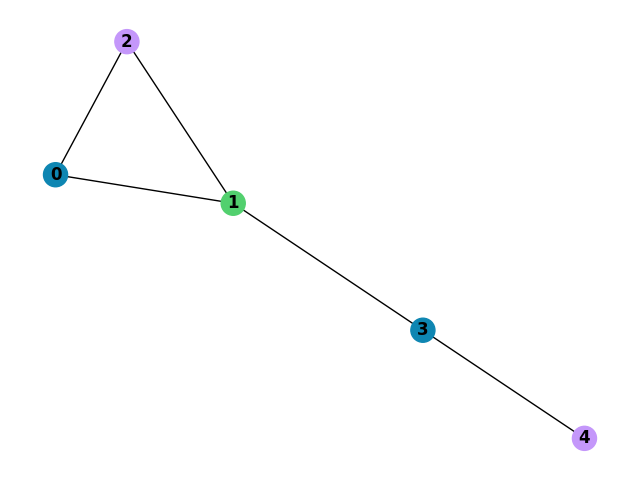
\includegraphics[width=10cm, keepaspectratio]{Colored Camel_files/Colored Camel_60_5.png}
\end{figure}


    \begin{tcolorbox}[breakable, size=fbox, boxrule=1pt, pad at break*=1mm,colback=cellbackground, colframe=cellborder]
\prompt{In}{incolor}{18}{\boxspacing}
\begin{Verbatim}[commandchars=\\\{\}]
\PY{n}{risolvi} \PY{n}{problema\PYZus{}2}\PY{o}{;;}
\end{Verbatim}
\end{tcolorbox}

 \begin{figure}[H]
     \centering
     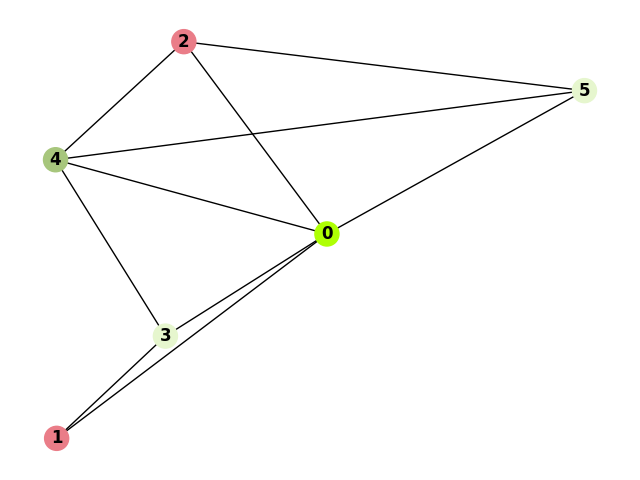
\includegraphics[width=12cm, keepaspectratio]{Colored Camel_files/Colored Camel_61_6.png}
 \end{figure}

    
        
    \begin{tcolorbox}[breakable, size=fbox, boxrule=1pt, pad at break*=1mm,colback=cellbackground, colframe=cellborder]
\prompt{In}{incolor}{19}{\boxspacing}
\begin{Verbatim}[commandchars=\\\{\}]
\PY{n}{risolvi} \PY{n}{problema\PYZus{}2\PYZus{}err}\PY{o}{;;}
\end{Verbatim}
\end{tcolorbox}

    \begin{Verbatim}[commandchars=\\\{\}, frame=single, framerule=2mm, rulecolor=\color{outerrorbackground}]
\textcolor{ansi-red}{Exception: NumeroColoriInsifficiente.}
    \end{Verbatim}

    \begin{tcolorbox}[breakable, size=fbox, boxrule=1pt, pad at break*=1mm,colback=cellbackground, colframe=cellborder]
\prompt{In}{incolor}{20}{\boxspacing}
\begin{Verbatim}[commandchars=\\\{\}]
\PY{n}{risolvi} \PY{n}{problema\PYZus{}6}\PY{o}{;;}
\end{Verbatim}
\end{tcolorbox}

    \begin{figure}[H]
        \centering
        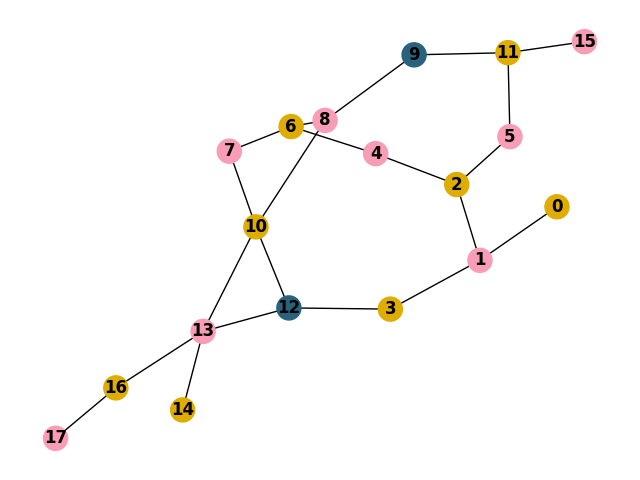
\includegraphics[width=15cm, keepaspectratio]{Colored Camel_files/Colored Camel_63_18.png}

    \end{figure}

    

        
    \begin{tcolorbox}[breakable, size=fbox, boxrule=1pt, pad at break*=1mm,colback=cellbackground, colframe=cellborder]
\prompt{In}{incolor}{21}{\boxspacing}
\begin{Verbatim}[commandchars=\\\{\}]
\PY{n}{risolvi} \PY{n}{problema\PYZus{}4}\PY{o}{;;}
\end{Verbatim}
\end{tcolorbox}

    \begin{figure}[H]
        \centering
        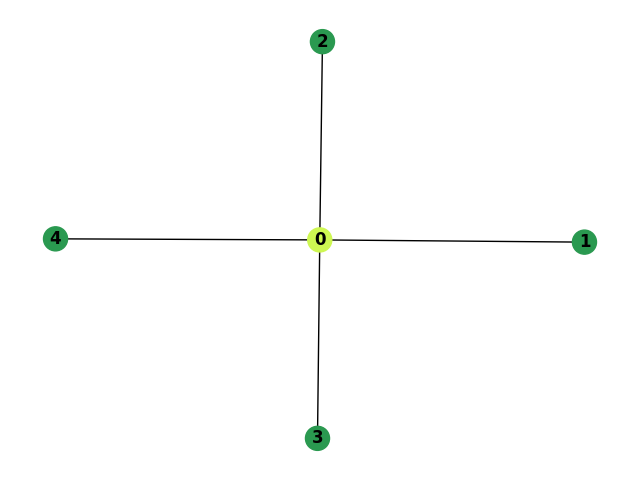
\includegraphics[width=10cm, keepaspectratio]{Colored Camel_files/Colored Camel_64_5.png}
    \end{figure}



\section{\texorpdfstring{I \emoji{broken-heart} Jupyter
}{I \emoji{broken-heart} Jupyter }}\label{i-jupyter}

    Oltre alla stesura di questo notebook (che presenta una versione
certamente funzionante, seppur minimale, dell'algoritmo) ho riscritto
tutto il progetto in modo tale che sia compilabile ed eseguibile anche
da terminale approfondendo anche altri argomenti e funzionalità del
linguaggio.

È disponibili all'interno della cartella \texttt{progetto} e presenta la
seguente struttura:

    \begin{figure}
\centering
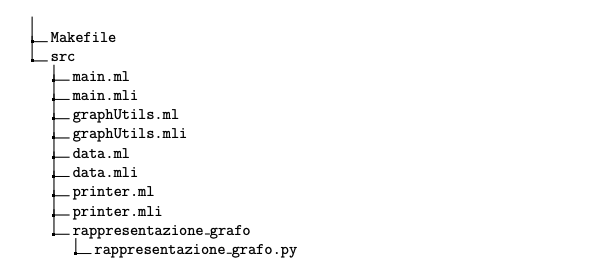
\includegraphics{Colored Camel_files/struttura.png}
\caption{Schermata\%202022-07-31\%20alle\%2009.57.16.png}
\end{figure}

    \begin{itemize}
\tightlist
\item
  \texttt{Makefile}: utilizzato per compilare il progetto e generare
  l'eseguibile
\item
  \texttt{main}: contiene la funzione principale che si occupa di
  avviare la risoluzione dei problemi e di gestire le scelte
  dell'utente.
\item
  \texttt{graphUtils}: insieme di funzioni per risolvere il problema
  della colorazione.
\item
  \texttt{data}: insieme di problemi per testare il corretto
  funzionamento del progetto. Questi possono essere aggiunti e rimossi
  in modo semplice ed efficiente.
\item
  \texttt{printer}: insieme di funzioni ed espressioni per stampare a
  video menù ed altri elementi con anche la presenza di colori ed emoji
  \emoji{rocket}.
\item
  \texttt{rappresentazione\_grafo}: script in python per rappresentare a
  video (in modo interattivo) un grafo.
\end{itemize}

    \hypertarget{makefile}{%
\subsection{\texorpdfstring{Makefile }{Makefile }}\label{makefile}}

    È il file utilizzato per la compilazione del progetto che avviene
tramite il comando \texttt{make}. Qualora un file venga modificato,
questo permette di non dover ricompilare tutto il progetto ma solo
quello che è stato cambiato. In una prima fase compila tutti i file
\texttt{.ml} con i relativi \texttt{.mli}, generando 2 altri file:

\begin{itemize}
\tightlist
\item
  \texttt{.cmi}: interfacce compilate utili per il corretto
  funzionamento dell'estensione OCaml in Visual Studio Code e per la
  corretta compilazione degli altri file. Questi vengono lasciati
  all'interno della cartella \texttt{src} e non spostati in quella
  designata alla fase di building per permettere il corretto
  funzionamento delle estensioni dell'editor.
\item
  \texttt{.cmo}: file oggetto che verranno poi spostati nella cartella
  \texttt{build} per essere utilizzati nella fase di linking.
\end{itemize}

Quindi, ogni file \texttt{.cmo} dipende dai relativi file \texttt{.ml} e
.\texttt{mli}. Successivamente, avvia la fase di linking unendo insieme
tutti i file \texttt{.cmo} e generando l'eseguibile \texttt{exe} nella
cartella \texttt{bin}. All'interno di quest'ultima viene copiato anche
lo script python per permettere il corretto funzionamento del progetto.

    \begin{Shaded}
\begin{Highlighting}[]
\DataTypeTok{cc }\CharTok{=}\StringTok{ ocamlc}
\DataTypeTok{cflags }\CharTok{=}\StringTok{ {-}c}
\DataTypeTok{cinclude }\CharTok{=}\StringTok{ {-}I src}

\DataTypeTok{srcdir }\CharTok{=}\StringTok{ src}
\DataTypeTok{buildir }\CharTok{=}\StringTok{ build}
\DataTypeTok{bindir }\CharTok{=}\StringTok{ bin}

\DataTypeTok{target }\CharTok{=}\StringTok{ }\CharTok{$(}\DataTypeTok{bindir}\CharTok{)}\StringTok{/exe}

\OtherTok{.PHONY:}\DataTypeTok{ clear}

\DecValTok{all:}\DataTypeTok{ cartelle }\CharTok{$(}\DataTypeTok{target}\CharTok{)}


\DecValTok{$(target):}
\DataTypeTok{ }\CharTok{$(}\DataTypeTok{buildir}\CharTok{)}\DataTypeTok{/graphUtils.cmo }\CharTok{$(}\DataTypeTok{buildir}\CharTok{)}\DataTypeTok{/printer.cmo }\CharTok{$(}\DataTypeTok{buildir}\CharTok{)}\DataTypeTok{/data.cmo }\CharTok{$(}\DataTypeTok{buildir}\CharTok{)}\DataTypeTok{/main.cmo}
    \CharTok{$(}\DataTypeTok{cc}\CharTok{)}\NormalTok{ {-}o }\CharTok{$@} \CharTok{$\^{}}
\NormalTok{    cp }\CharTok{$(}\DataTypeTok{srcdir}\CharTok{)}\NormalTok{/rappresentazione\_grafo/rappresentazione\_grafo.py }\CharTok{$(}\DataTypeTok{bindir}\CharTok{)}


\DecValTok{$(buildir)/graphUtils.cmo:}\DataTypeTok{ }\CharTok{$(}\DataTypeTok{srcdir}\CharTok{)}\DataTypeTok{/graphUtils.mli }\CharTok{$(}\DataTypeTok{srcdir}\CharTok{)}\DataTypeTok{/graphUtils.ml }
    \CharTok{$(}\DataTypeTok{cc}\CharTok{)} \CharTok{$(}\DataTypeTok{cinclude}\CharTok{)} \CharTok{$(}\DataTypeTok{cflags}\CharTok{)} \CharTok{$\^{}}
\NormalTok{    mv }\CharTok{$(}\DataTypeTok{srcdir}\CharTok{)}\NormalTok{/graphUtils.cmo }\CharTok{$(}\DataTypeTok{buildir}\CharTok{)}
    
\DecValTok{$(buildir)/printer.cmo:}\DataTypeTok{ }\CharTok{$(}\DataTypeTok{srcdir}\CharTok{)}\DataTypeTok{/printer.mli }\CharTok{$(}\DataTypeTok{srcdir}\CharTok{)}\DataTypeTok{/printer.ml}
    \CharTok{$(}\DataTypeTok{cc}\CharTok{)} \CharTok{$(}\DataTypeTok{cinclude}\CharTok{)} \CharTok{$(}\DataTypeTok{cflags}\CharTok{)} \CharTok{$\^{}}
\NormalTok{    mv }\CharTok{$(}\DataTypeTok{srcdir}\CharTok{)}\NormalTok{/printer.cmo }\CharTok{$(}\DataTypeTok{buildir}\CharTok{)}

\DecValTok{$(buildir)/data.cmo:}\DataTypeTok{ }\CharTok{$(}\DataTypeTok{srcdir}\CharTok{)}\DataTypeTok{/data.mli }\CharTok{$(}\DataTypeTok{srcdir}\CharTok{)}\DataTypeTok{/data.ml}
    \CharTok{$(}\DataTypeTok{cc}\CharTok{)} \CharTok{$(}\DataTypeTok{cinclude}\CharTok{)} \CharTok{$(}\DataTypeTok{cflags}\CharTok{)} \CharTok{$\^{}}
\NormalTok{    mv }\CharTok{$(}\DataTypeTok{srcdir}\CharTok{)}\NormalTok{/data.cmo }\CharTok{$(}\DataTypeTok{buildir}\CharTok{)}

\DecValTok{$(buildir)/main.cmo:}\DataTypeTok{ }\CharTok{$(}\DataTypeTok{srcdir}\CharTok{)}\DataTypeTok{/main.mli }\CharTok{$(}\DataTypeTok{srcdir}\CharTok{)}\DataTypeTok{/main.ml}
    \CharTok{$(}\DataTypeTok{cc}\CharTok{)} \CharTok{$(}\DataTypeTok{cinclude}\CharTok{)} \CharTok{$(}\DataTypeTok{cflags}\CharTok{)} \CharTok{$\^{}}
\NormalTok{    mv }\CharTok{$(}\DataTypeTok{srcdir}\CharTok{)}\NormalTok{/main.cmo }\CharTok{$(}\DataTypeTok{buildir}\CharTok{)}


\DecValTok{cartelle:}\DataTypeTok{ }\CharTok{$(}\DataTypeTok{buildir}\CharTok{)}\DataTypeTok{ }\CharTok{$(}\DataTypeTok{bindir}\CharTok{)}

\DecValTok{$(buildir):}
\NormalTok{    mkdir {-}p }\CharTok{$@}

\DecValTok{$(bindir):}
\NormalTok{    mkdir {-}p }\CharTok{$@}

\DecValTok{clear:}
\NormalTok{    rm {-}f }\CharTok{$(}\DataTypeTok{buildir}\CharTok{)}\NormalTok{/*.cmo}
\NormalTok{    rm {-}f }\CharTok{$(}\DataTypeTok{bindir}\CharTok{)}\NormalTok{/*}
\NormalTok{    rm {-}f }\CharTok{$(}\DataTypeTok{srcdir}\CharTok{)}\NormalTok{/*.cmi}
\end{Highlighting}
\end{Shaded}

\emph{Contenuto di Makfile}\\

    Un esempio pratico di come eseguire la fase di compilazione:

    \begin{tcolorbox}[breakable, size=fbox, boxrule=1pt, pad at break*=1mm,colback=cellbackground, colframe=cellborder]
\prompt{In}{incolor}{29}{\boxspacing}
\begin{Verbatim}[commandchars=\\\{\}]
\PY{c}{(*}\PY{c}{ compilazione del progetto }\PY{c}{*)}
\PY{n+nn}{Process}\PY{p}{.}\PY{n}{sh} \PY{l+s+s2}{\PYZdq{}}\PY{l+s+s2}{cd progetto; make; ls \PYZhy{}LR}\PY{l+s+s2}{\PYZdq{}}\PY{o}{;;}

\PY{c}{(*}\PY{c}{ pulizia e rimozione dei file compilati}\PY{c}{*)}
\PY{n+nn}{Process}\PY{p}{.}\PY{n}{sh} \PY{l+s+s2}{\PYZdq{}}\PY{l+s+s2}{cd progetto; make clear; ls \PYZhy{}LR}\PY{l+s+s2}{\PYZdq{}}\PY{o}{;;}
\end{Verbatim}
\end{tcolorbox}

  \begin{tcolorbox}[breakable, size=fbox, boxrule=.5pt, pad at break*=1mm, opacityfill=0]
\prompt{Out}{outcolor}{29}{\boxspacing}
    \begin{Verbatim}[commandchars=\\\{\}]
ocamlc -I src -c src/graphUtils.mli src/graphUtils.ml
mv src/graphUtils.cmo build
ocamlc -I src -c src/printer.mli src/printer.ml
mv src/printer.cmo build
ocamlc -I src -c src/data.mli src/data.ml
mv src/data.cmo build
ocamlc -I src -c src/main.mli src/main.ml
mv src/main.cmo build
ocamlc -o bin/exe build/graphUtils.cmo build/printer.cmo build/data.cmo
build/main.cmo
cp src/rappresentazione\_grafo/rappresentazione\_grafo.py bin

    \end{Verbatim}
\end{tcolorbox}
        
     \begin{tcolorbox}[breakable, size=fbox, boxrule=.5pt, pad at break*=1mm, opacityfill=0]
\prompt{Out}{outcolor}{29}{\boxspacing}
    \begin{Verbatim}[commandchars=\\\{\}]
rm -f build/*.cmo
rm -f bin/*
rm -f src/*.cmi
    \end{Verbatim}
\end{tcolorbox}

        
    \hypertarget{printer}{%
\subsection{\texorpdfstring{Printer }{Printer }}\label{printer}}

    In questo file risiedono tutte le funzioni e dichiarazioni che
gestiscono la stampa a video. Vi è una definizione di stringhe per
stampare su terminale caratteri colorati (rosso, verde, blu, ecc.),
elementi in grassetto ed emoji (a patto che questo li supporti). La
funzione più degna di nota è \texttt{stampa\_problema} che, dato un
problema, stampa a schermo tutti i suoi dati:

\begin{itemize}
\tightlist
\item
  il grafo
\item
  il nodo di partenza
\item
  il massimo numero di colori \(N\)
\end{itemize}

    \begin{Shaded}
\begin{Highlighting}[]
\KeywordTok{type}\NormalTok{ colore = Colore }\KeywordTok{of} \DataTypeTok{string}\NormalTok{ ;;}

\CommentTok{(* normali *)}
\KeywordTok{let}\NormalTok{ rosso = Colore }\StringTok{" }\CharTok{\textbackslash{}027}\StringTok{[31 m"}\NormalTok{;;}
\KeywordTok{let}\NormalTok{ verde = Colore }\StringTok{" }\CharTok{\textbackslash{}027}\StringTok{[32 m"}\NormalTok{;;}
\KeywordTok{let}\NormalTok{ ciano = Colore }\StringTok{" }\CharTok{\textbackslash{}027}\StringTok{[36 m"}\NormalTok{;;}
\KeywordTok{let}\NormalTok{ bianco = Colore }\StringTok{" }\CharTok{\textbackslash{}027}\StringTok{[0 m"}\NormalTok{;;}

\CommentTok{(* grassetto *)}
\KeywordTok{let}\NormalTok{ rosso\_b = Colore }\StringTok{" }\CharTok{\textbackslash{}027}\StringTok{[31;1 m"}\NormalTok{;;}
\KeywordTok{let}\NormalTok{ verde\_b = Colore }\StringTok{" }\CharTok{\textbackslash{}027}\StringTok{[32;1 m"}\NormalTok{;;}
\KeywordTok{let}\NormalTok{ ciano\_b = Colore }\StringTok{" }\CharTok{\textbackslash{}027}\StringTok{[36;1 m"}\NormalTok{;;}
\KeywordTok{let}\NormalTok{ bianco\_b = Colore }\StringTok{" }\CharTok{\textbackslash{}027}\StringTok{[0;1 m"}\NormalTok{;;}

\CommentTok{(* valore di reset per stampare normalmente *)}
\KeywordTok{let}\NormalTok{ reset = bianco ;;}
\end{Highlighting}
\end{Shaded}

\emph{Alcune definizioni di colori}

\begin{Shaded}
\begin{Highlighting}[]
\KeywordTok{let}\NormalTok{ stampa\_problema (Problema((Grafo }\DataTypeTok{succ}\NormalTok{), partenza, maxColori)) =}
\NormalTok{    print\_colore rosso\_b }\StringTok{" Partenza : "}\NormalTok{;}
    \DataTypeTok{print\_int}\NormalTok{ partenza ; print\_colore rosso\_b }\StringTok{" Max Colori : "}\NormalTok{;}
    \DataTypeTok{print\_int}\NormalTok{ maxColori ; }\DataTypeTok{print\_string} \StringTok{"}\CharTok{\textbackslash{}n\textbackslash{}n}\StringTok{"}\NormalTok{;}
    \KeywordTok{let} \KeywordTok{rec}\NormalTok{ search visitati = }\KeywordTok{function} \CommentTok{(* frontiera *)}
\NormalTok{        [] {-}\textgreater{} }\DataTypeTok{print\_string} \StringTok{"}\CharTok{\textbackslash{}n}\StringTok{"} \CommentTok{(* caso base , stampa \textbackslash{}n*)}
\NormalTok{      | nodo :: coda {-}\textgreater{} }\CommentTok{(* stampa nodo e vicini *)}
        \KeywordTok{if} \DataTypeTok{List}\NormalTok{.mem nodo visitati }\CommentTok{(* ignora nodi visti *)}
            \KeywordTok{then}
\NormalTok{                search visitati coda}
        \KeywordTok{else} \CommentTok{(* stampa il nodo e vicini .*)}
\NormalTok{           (print\_colore verde\_b (}\DataTypeTok{string\_of\_int}\NormalTok{ nodo);}
\NormalTok{            print\_colore bianco\_b }\StringTok{" {-}\textgreater{} "}\NormalTok{;}
\NormalTok{            stampa\_lista (}\DataTypeTok{succ}\NormalTok{ nodo);}
\NormalTok{            search (visitati@[nodo])(coda@(}\DataTypeTok{succ}\NormalTok{ nodo)))}

    \KeywordTok{in}\NormalTok{ search [] [partenza] }\CommentTok{(* avvia la ricorsione *)}
\end{Highlighting}
\end{Shaded}

\emph{Codice della funzione \texttt{stampa\_problema}}

    \begin{figure}
\centering
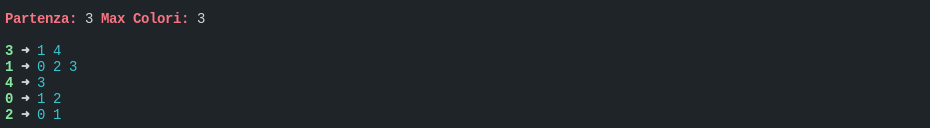
\includegraphics{Colored Camel_files/grafoterminale.png}
\caption{grafoTerminale.png}
\end{figure}

\emph{Output della funzione}

    \hypertarget{data}{%
\subsection{\texorpdfstring{Data }{Data }}\label{data}}

    In questo file ci sono tutte le definizioni dei problemi utilizzati come
test per verificare il corretto funzionamento dell'algoritmo di
colorazione; una funzione che permette di stampare un menù con alcune
informazioni come la descrizione dei grafi, gli ID unici, ecc; ed una
funzione che dato un numero (ID), ritorna uno dei precedenti problemi. È
anche presente una lista (\texttt{problemi}) che contiene tutti i
problemi disponibili con una descrizione (una coppia
\texttt{(problema,\ string)}). È questa che permette di aggiungere e
togliere elementi in maniera semplice senza dover modificare alcuna
funzione.

    \begin{Shaded}
\begin{Highlighting}[]
\KeywordTok{let}\NormalTok{ problemi = [}
\NormalTok{    ( problema\_1 , }\StringTok{" Grafo 1"}\NormalTok{) ;}
\NormalTok{    ( problema\_2 , }\StringTok{" Grafo 2 con numero sufficiente di colori "}\NormalTok{) ;}
\NormalTok{    ( problema\_2\_err , }\StringTok{" Grafo 2 con colori insufficienti "}\NormalTok{) ;}
\NormalTok{    ( problema\_3 , }\StringTok{" Grafo 3"}\NormalTok{) ;}
\NormalTok{    ( problema\_4 , }\StringTok{" Grafo 4"}\NormalTok{)}
\NormalTok{];;}
\end{Highlighting}
\end{Shaded}

\emph{Parte della lista \texttt{problemi}}

    \begin{figure}
\centering
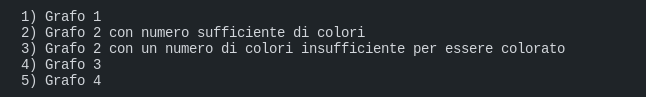
\includegraphics{Colored Camel_files/descrizionegrafi.png}
\caption{descrizione\_grafi.png}
\end{figure}

\emph{Output per la selezione del problema da risolvere}

    Infine, la funzione \texttt{scegli\_problema} che, dato un ID, ritorna
il relativo problema. È interessante notare come per selezionare un dato
problema non viene scorsa ricorsivamente tutta la lista, ma quest'ultima
viene convertita in un \texttt{Array} per poter utilizzare il metodo
\texttt{get} per accedere all'\emph{i}-esima posizione. Vengono
effettuati alcuni controlli sull'input: viene controllato se l'ID
passato è valido (non superi per eccesso, o per difetto gli ID mostrati
a video) e nel caso solleva un'eccezione (verrà utilizzata nella
funzione \texttt{main} per segnalare il problema).

    \begin{Shaded}
\begin{Highlighting}[]
\KeywordTok{let}\NormalTok{ scegli\_problema id\_problema =}
    \KeywordTok{let}\NormalTok{ array\_tmp = }\DataTypeTok{Array}\NormalTok{.of\_list problemi }\KeywordTok{in} \CommentTok{(* lista in array *)}
        \KeywordTok{if}\NormalTok{ id\_problema \textgreater{} }\DataTypeTok{Array}\NormalTok{.length array\_tmp || id\_problema \textless{} }\DecValTok{1}
          \KeywordTok{then}
            \DataTypeTok{raise}\NormalTok{ SceltaErrata }\CommentTok{(* lancia un \textquotesingle{} eccezione *)}
        \KeywordTok{else}
            \DataTypeTok{fst}\NormalTok{ ( }\DataTypeTok{Array}\NormalTok{.get array\_tmp ( id\_problema }\DecValTok{{-}1}\NormalTok{) ) }
\NormalTok{;;}
\end{Highlighting}
\end{Shaded}

\emph{Codice della funzione scegli\_problema}

    \hypertarget{graphutils}{%
\subsection{\texorpdfstring{GraphUtils
}{GraphUtils }}\label{graphutils}}

    Nel file \texttt{graphUtils.ml} possiamo trovare tutte le funzioni
implementate ed analizzate fin ora che riguardano l'algoritmo di
colorazione. La parte delle \emph{funzioni ausiliarie} è esattamente
identica, l'unica differenza possiamo trovarla nella funzione
\texttt{risolvi}, dove sono state apportate alcune piccole modifiche per
permettere l'esecuzione da riga di comando:

\begin{itemize}
\tightlist
\item
  Ora ritorna il risultato (la lista \texttt{colorati}) e non stampa o
  mostra a schermo più nulla, sarà un problema del main,
\item
  Lo script python non viene più fatto partire qui dentro ma sarà
  compito del main avviarlo.
\end{itemize}

\newpage

    \begin{Shaded}
\begin{Highlighting}[]
\KeywordTok{let}\NormalTok{ risolvi (Problema ((Grafo }\DataTypeTok{succ}\NormalTok{), partenza, maxColori)) =}
  \KeywordTok{let}\NormalTok{ risultato = inizializza\_risultato (Grafo }\DataTypeTok{succ}\NormalTok{) partenza }\KeywordTok{in}  
  \KeywordTok{let} \KeywordTok{rec}\NormalTok{ esplora visitati colorati = }
    \KeywordTok{function} \CommentTok{(*frontiera*)}
\NormalTok{        []            {-}\textgreater{}          }\CommentTok{(*fine delle ricorsione*)}
\NormalTok{          (salva\_grafo\_colorato (Grafo }\DataTypeTok{succ}\NormalTok{) colorati; colorati)}

\NormalTok{      | nodo::coda    {-}\textgreater{}           }\CommentTok{(*caso ricorsivo, continua a colorare*)}
        \KeywordTok{if} \DataTypeTok{List}\NormalTok{.mem nodo visitati              }\CommentTok{(*se il nodo è già stato visitato*)}
          \KeywordTok{then}\NormalTok{ esplora visitati colorati coda     }\CommentTok{(* ignora il nodo e continua*)}
        
        \KeywordTok{else} 
          \CommentTok{(*continua con la ricorsione espandendo i nodi vicini al nodo*)}
\NormalTok{          esplora }
\NormalTok{                (visitati@[nodo])      }\CommentTok{(*aggiunge il nodo attuale ai visitati*)}
\NormalTok{                (incrementa\_colore\_nodi } 
\NormalTok{                     colorati} 
\NormalTok{                     (}\DataTypeTok{succ}\NormalTok{ nodo)}
\NormalTok{                     (get\_colore nodo colorati) maxColori) }
\NormalTok{                (coda@(}\DataTypeTok{succ}\NormalTok{ nodo))     }
\CommentTok{                (*espande i vicini del nodo attuale e li aggiunge alla frontiera*)}
      
  \KeywordTok{in}\NormalTok{ esplora [] risultato [partenza]}
\NormalTok{;;}
\end{Highlighting}
\end{Shaded}

\emph{Codice della funzione \texttt{risolvi} in graphUtils.ml}

    Qui vengono anche definiti i tipi \texttt{grafo} e \texttt{problema},
con i relativi costruttori di tipo \texttt{Grafo} e \texttt{Problema}.
Viene anche creata l'eccezione \texttt{NumeroColoriInsufficiente} che
servirà per segnalare che il dato problema non è risolvibile per il
numero insufficiente di colori selezionato.

    \hypertarget{main}{%
\subsection{\texorpdfstring{Main }{Main }}\label{main}}

    In questo file è presente la funzione principale \texttt{main} che si
occupa di gestire tutto il flusso del programma: stampa il menu
iniziale, fa scegliere all'utente su quale problema testare l'algoritmo
di colorazione, avvia la risoluzione del problema selezionato, stampa il
risultato ed avvia lo script python.

    \begin{Shaded}
\begin{Highlighting}[]
\KeywordTok{let}\NormalTok{ main () =}
\NormalTok{    stampa\_logo ();}
\NormalTok{    stampa\_problemi\_disponibili ();}

    \KeywordTok{let}\NormalTok{ dati =}
        \KeywordTok{let} \KeywordTok{rec}\NormalTok{ aux () = }\CommentTok{(* utente sceglie il problema *)}
            \KeywordTok{try} \CommentTok{(* controllo input valido *)}
\NormalTok{                scegli\_problema ( scelta () )}
            \KeywordTok{with}\NormalTok{ SceltaErrata {-}\textgreater{}}
\NormalTok{                aux ()}
        \KeywordTok{in}\NormalTok{ aux ()}
  \KeywordTok{in} \KeywordTok{let}\NormalTok{ avvia\_colorazione (Problema(g, partenza, maxColori)) =}
    \DataTypeTok{print\_string} \StringTok{"}\CharTok{\textbackslash{}n}\StringTok{Il Problema selezionato : }\CharTok{\textbackslash{}n\textbackslash{}n}\StringTok{"}\NormalTok{;}
\NormalTok{    stampa\_problema ( Problema (g , partenza , maxColori ) ) ;}
    \DataTypeTok{print\_string} \StringTok{" Coloro ...\textbackslash{} n}\CharTok{\textbackslash{}n}\StringTok{"}\NormalTok{;}

    \CommentTok{(* colora il grafo *)}
    \KeywordTok{let}\NormalTok{ colorati = risolvi (Problema(g, partenza, maxColori)) }\KeywordTok{in}
\NormalTok{        stampa\_nodi\_colorati colorati;}\CommentTok{(*stampa il grafo colorato*)}
\NormalTok{        salva\_grafo\_colorato g colorati;}\CommentTok{(*salva grafo colorato*)}
\NormalTok{        avvia\_python () }\CommentTok{(* avvia python *)}

    \KeywordTok{in} \CommentTok{(* con un grafo scelto , lo colora *)}
        \KeywordTok{try}
\NormalTok{            avvia\_colorazione dati}
        \KeywordTok{with}\NormalTok{ NumeroColoriInsufficiente {-}\textgreater{}}
\NormalTok{            stampa\_errore ()}
\NormalTok{;;}
\end{Highlighting}
\end{Shaded}

\emph{Parte del codice del file \texttt{main.ml}}

    Alla riga \(2 - 3\) viene stampato sul terminale il logo iniziale e
tutti i problemi disponibili per testare l'algoritmo. Nelle successive
righe (\(5 - 27\)) vengono definite alcune funzioni ausiliarie per
mettere in pratica i comportamenti descritti prima:

\begin{itemize}
\tightlist
\item
  \texttt{dati}: rimane fermo sulla scelta del problema fin quando
  l'utente non seleziona un ID esistente. Una volta selezionato un ID
  valido conterrà il problema scelto.
\item
  \texttt{avvia\_colorazione}: stampa alcune informazioni utili
  all'utente per poi colorare il grafo, salvarlo su file e avviare lo
  script python. Qui vengono anche gestite le possibili eccezioni.
\end{itemize}

    Nelle prime righe del file vengono inclusi gli altri codici descritti
nelle precedenti sezioni con:

\begin{Shaded}
\begin{Highlighting}[]
\KeywordTok{open}\NormalTok{ Printer ;;}
\KeywordTok{open}\NormalTok{ GraphUtils ;;}
\KeywordTok{open}\NormalTok{ Data ;;}
\end{Highlighting}
\end{Shaded}

\emph{Inclusione degli altri file \texttt{.ml}}

    \hypertarget{python}{%
\subsection{\texorpdfstring{Python }{Python }}\label{python}}

    All'interno del progetto è anche presente un breve script in python che
verrà avviato una volta risolto il problema della colorazione. Questo
script legge il file \texttt{.data} generato da OCaml (contiene il grafo
ed i colori di ogni nodo) e lo rappresenta all'interno di una finestra
in modo interattivo e soprattutto più comprensibile rispetto alla
visualizzazione su terminale.

Presenta 2 modalità di utilizzo:

\begin{itemize}
\tightlist
\item
  \textbf{notebook}: in questa modalità produce in output un'immagine
  compatibile con i notebook di jupyter. Sarà poi compito di OCaml
  andare ad importarla e disegnarla.
\item
  \textbf{eseguibile}: questa modalità viene utilizzata quando lo script
  è invocato dal progetto compilato, genera una pagina HTML, che verrà
  aperta in automatico, con la visualizzazione interattiva del grafo
  colorato.
\end{itemize}

    \begin{Shaded}
\begin{Highlighting}[]
\ImportTok{import}\NormalTok{ networkx }\ImportTok{as}\NormalTok{ nx}
\ImportTok{from}\NormalTok{ pyvis.network }\ImportTok{import}\NormalTok{ Network}
\ImportTok{import}\NormalTok{ matplotlib.pyplot }\ImportTok{as}\NormalTok{ plt}


\KeywordTok{def}\NormalTok{ main(args):}
    \CommentTok{\# controlla che il nome del file sia stato passato}
    \ControlFlowTok{if} \BuiltInTok{len}\NormalTok{(args) }\OperatorTok{\textless{}=} \DecValTok{0}\NormalTok{: }\ControlFlowTok{return}

\NormalTok{    fname }\OperatorTok{=}\NormalTok{ args[}\DecValTok{0}\NormalTok{]}
\NormalTok{    in\_jupyter }\OperatorTok{=} \VariableTok{True} \ControlFlowTok{if} \BuiltInTok{len}\NormalTok{(args) }\OperatorTok{\textgreater{}=} \DecValTok{2} \ControlFlowTok{else} \VariableTok{False}
    
\NormalTok{    collegamenti }\OperatorTok{=}\NormalTok{ []}
\NormalTok{    nodi }\OperatorTok{=}\NormalTok{ []}
\NormalTok{    colori }\OperatorTok{=}\NormalTok{ []}

    \CommentTok{\# lettura dei dati da file}
    \ControlFlowTok{with} \BuiltInTok{open}\NormalTok{(fname, }\StringTok{\textquotesingle{}r\textquotesingle{}}\NormalTok{) }\ImportTok{as}\NormalTok{ f:}
        \ControlFlowTok{for}\NormalTok{ text }\KeywordTok{in}\NormalTok{ f.readlines():}
\NormalTok{            text }\OperatorTok{=}\NormalTok{ text.strip(}\StringTok{"}\CharTok{\textbackslash{}n}\StringTok{"}\NormalTok{) }\CommentTok{\# elimina i vari \textbackslash{}n nel file}
            \ControlFlowTok{if}\NormalTok{ text }\OperatorTok{!=} \StringTok{\textquotesingle{}\textquotesingle{}}\NormalTok{:  }\CommentTok{\# controlla che la riga sia valida}
\NormalTok{                nodo, vicini, colore  }\OperatorTok{=}\NormalTok{ text.split(}\StringTok{","}\NormalTok{)}
                
\NormalTok{                vicini }\OperatorTok{=}\NormalTok{ vicini.split(}\StringTok{" "}\NormalTok{)}
\NormalTok{                colori.append(}\BuiltInTok{int}\NormalTok{(colore))}
                
                \CommentTok{\# controlla se il nodo ha vicini}
                \ControlFlowTok{if}\NormalTok{ vicini[}\DecValTok{0}\NormalTok{] }\OperatorTok{!=} \StringTok{\textquotesingle{}\textquotesingle{}}\NormalTok{:  }
                    \CommentTok{\# crea gli archi del grafo}
                    \ControlFlowTok{for}\NormalTok{ vicino }\KeywordTok{in}\NormalTok{ vicini: }
\NormalTok{                        tmp }\OperatorTok{=}\NormalTok{ (}\BuiltInTok{int}\NormalTok{(nodo), }\BuiltInTok{int}\NormalTok{(vicino))}
\NormalTok{                        collegamenti.append(tmp) }
                        
    \CommentTok{\# controlla che abbia trovato tutti i nodi}
\NormalTok{    nodi }\OperatorTok{=}\NormalTok{ trova\_nodi(collegamenti)}
    \CommentTok{\# converte i colori da int a stringa hex per pyvis}
\NormalTok{    colori }\OperatorTok{=}\NormalTok{ aggiusta\_colori(colori) }

\NormalTok{    rappresenta\_grafo(nodi, collegamenti, colori, in\_jupyter)  }

\NormalTok{...}


\KeywordTok{def}\NormalTok{ rappresenta\_grafo (nodi, collegamenti, colori, in\_jupyter):}
    \ControlFlowTok{if}\NormalTok{ in\_jupyter:}
\NormalTok{        G }\OperatorTok{=}\NormalTok{ nx.Graph()}

\NormalTok{        G.add\_nodes\_from(nodi)}
\NormalTok{        G.add\_edges\_from(collegamenti)}

\NormalTok{        nx.draw(}
\NormalTok{            G, }
\NormalTok{            node\_color}\OperatorTok{=}\NormalTok{colori, }
\NormalTok{            with\_labels}\OperatorTok{=}\VariableTok{True}\NormalTok{, }
\NormalTok{            font\_weight}\OperatorTok{=}\StringTok{\textquotesingle{}bold\textquotesingle{}}
\NormalTok{        )}
\NormalTok{        plt.savefig(}\StringTok{"risultato.png"}\NormalTok{)}

    \ControlFlowTok{else}\NormalTok{:}
\NormalTok{        net }\OperatorTok{=}\NormalTok{ Network(}
\NormalTok{            width}\OperatorTok{=}\StringTok{\textquotesingle{}100\%\textquotesingle{}}\NormalTok{, }
\NormalTok{            height}\OperatorTok{=}\StringTok{\textquotesingle{}600px\textquotesingle{}}\NormalTok{, }
\NormalTok{            directed}\OperatorTok{=}\VariableTok{False}
\NormalTok{        )}

\NormalTok{        net.add\_nodes(}
\NormalTok{            nodi, }
\NormalTok{            label}\OperatorTok{=}\NormalTok{[}\SpecialStringTok{f"}\SpecialCharTok{\{x\}}\SpecialStringTok{"} \ControlFlowTok{for}\NormalTok{ x }\KeywordTok{in}\NormalTok{ nodi], }
\NormalTok{            color}\OperatorTok{=}\NormalTok{colori}
\NormalTok{        )}
\NormalTok{        net.add\_edges(collegamenti)}

\NormalTok{        net.toggle\_physics(}\VariableTok{True}\NormalTok{)}
\NormalTok{        net.inherit\_edge\_colors(}\VariableTok{False}\NormalTok{)}
\NormalTok{        net.write\_html(}\StringTok{\textquotesingle{}rappresentazione\_grafo.html\textquotesingle{}}\NormalTok{)}
\end{Highlighting}
\end{Shaded}

\emph{Parte delle funzioni dello script python}

    \begin{figure}
\centering
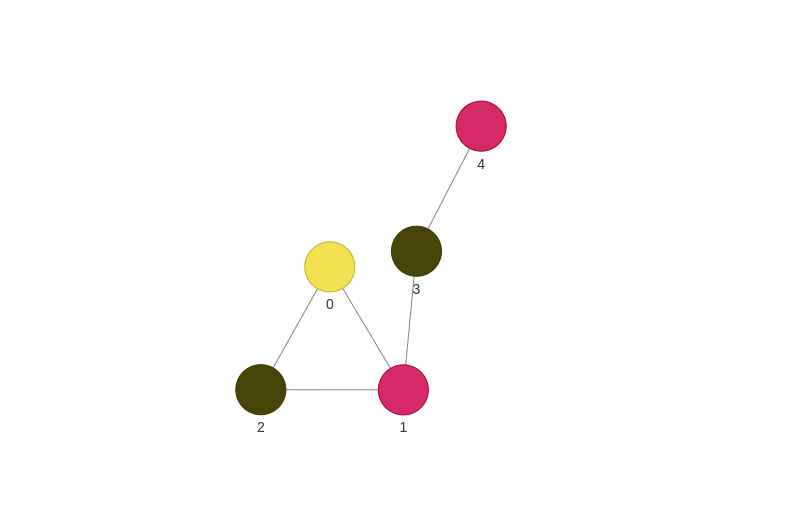
\includegraphics{Colored Camel_files/grafocoloratopy.png}
\caption{grafocoloratopy.png}
\end{figure}

\emph{Output dello script python}

    \hypertarget{dimostrazione-di-esecuzione}{%
\subsection{\texorpdfstring{Dimostrazione di Esecuzione
}{Dimostrazione di Esecuzione }}\label{dimostrazione-di-esecuzione}}

    Una volta compilato il progetto tramite il comando \texttt{make}, è
prima necessario spostarsi all'interno della cartella \texttt{bin} per
poi avviare l'eseguibile:

\begin{Shaded}
\begin{Highlighting}[]
\BuiltInTok{cd}\NormalTok{ bin}
\ExtensionTok{./exe}
\end{Highlighting}
\end{Shaded}

Verrà mostrato il menù iniziale e l'utente dovrà scegliere quale
problema utilizzare per testare l'algoritmo di colorazione. Se verrà
inserito un ID invalido si rimane bloccati in questa scelta fin quando
un ID corretto non verrà inserito. Una volta selezionato un ID valido
verrà stampato a video il grafo, con il nodo di partenza, il massimo
numero di colori ed il risultato della fase di colorazione. Infine verrà
avviato lo script python che aprirà una finestra con al suo interno il
grafo disegnato. Qualora l'utente selezionerà un problema che non è
colorabile, per via del numero insufficiente di colori, verrà mostrato a
video un messaggio di errore e non verrà avviato lo script python.

    \begin{figure}
\centering

\includegraphics{Colored Camel_files/menu.png}
\caption{menu.png}
\end{figure}

\emph{Menù iniziale}

    \begin{figure}
\centering
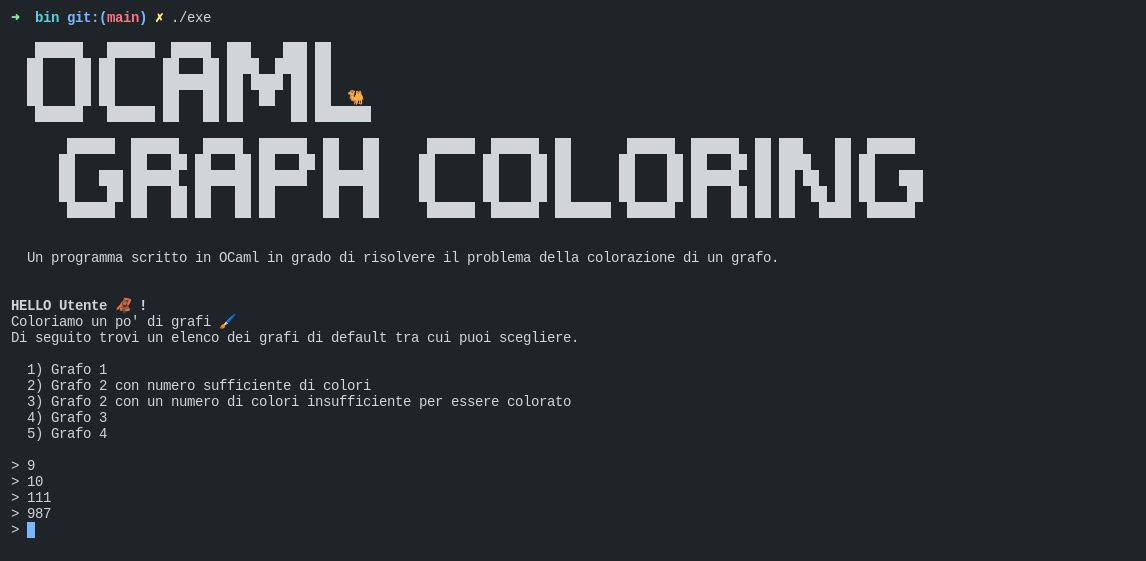
\includegraphics{Colored Camel_files/badid.png}
\caption{badid.png}
\end{figure}

\emph{Esempio di multiple scelte errate di ID}

    \begin{figure}
\centering
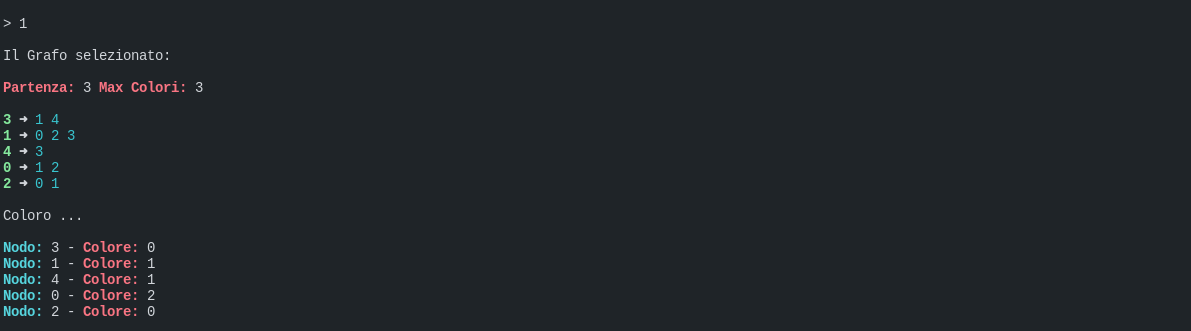
\includegraphics{Colored Camel_files/grafo1bin.png}
\caption{grafo1bin.png}
\end{figure}

\emph{Esempio di risoluzione di un problema}

    \begin{figure}
\centering
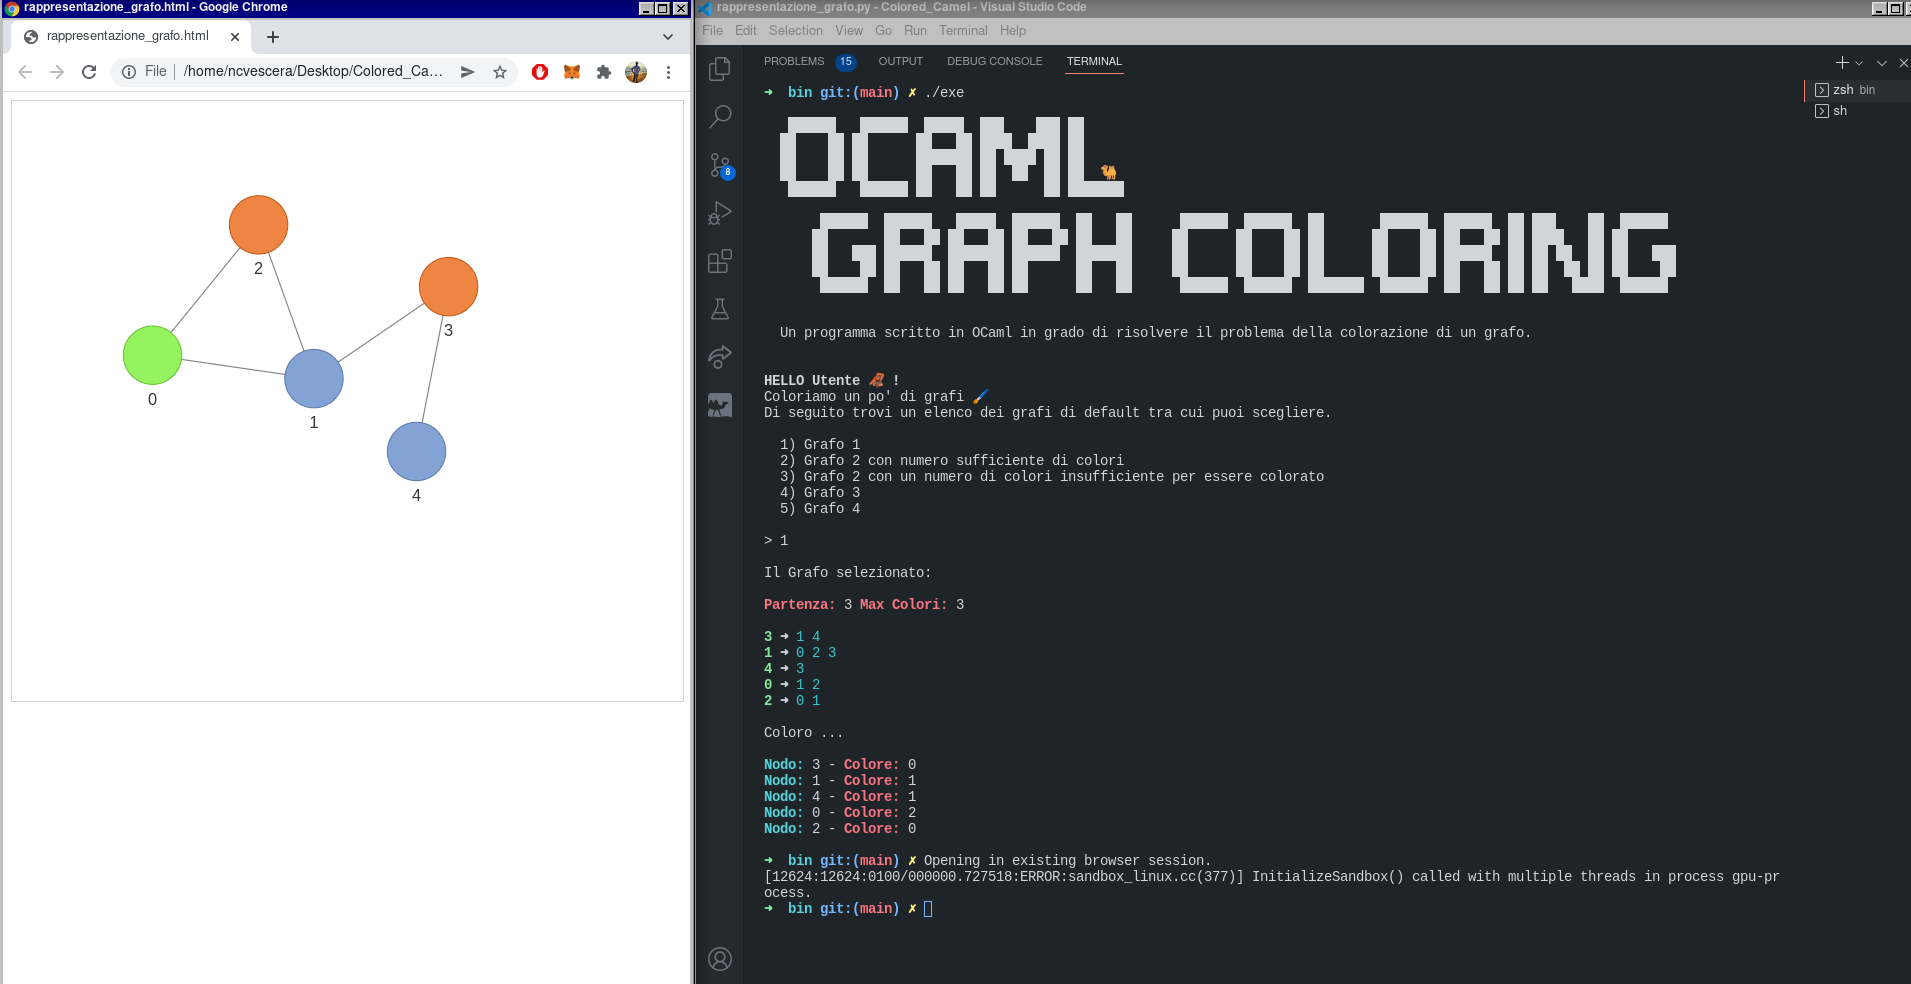
\includegraphics{Colored Camel_files/termgrafo.png}
\caption{termgrafo.png}
\end{figure}

\emph{Comportamento dello script python}

    \begin{figure}
\centering
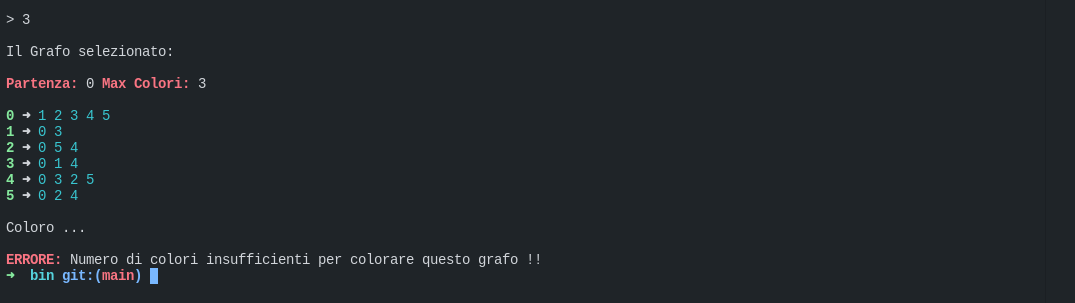
\includegraphics{Colored Camel_files/errore.png}
\caption{errore.png}
\end{figure}

\emph{Messaggio di errore per numero di colori insufficienti}

\newpage

\section{\texorpdfstring{Ambiente di Sviluppo \emoji{spouting-whale}
}{Ambiente di Sviluppo \emoji{spouting-whale}}}\label{ambiente-di-sviluppo}

    L'intero progetto è stato realizzato all'interno di un \textbf{container
docker} utilizzato come ambiente di sviluppo, questo mi ha permesso di
risparmiare notevole tempo nella configurazione e installazione di tutto
il software necessario al funzionamento di OCaml, ma soprattutto mi dà
la possibilità di avere un ambiente di sviluppo portatile che può essere
condiviso e avviato su qualunque macchina in pochissimo tempo.

Il tutto si basa sull'estensione
\href{https://code.visualstudio.com/docs/remote/containers}{Remote
Containers} per l'editor Visual Studio Code che permette di utilizzare
un container docker come un ambiente di sviluppo \emph{full-featured},
di poter aprire qualunque cartella all'interno del container e gestirla
tramite l'editor avendo a disposizione tutte le funzionalità che ci
offre. È anche possibile scegliere quali estensioni di VSCode andare ad
installare e utilizzare all'interno del nostro nuovo ambiente di
sviluppo.

Il file \texttt{devcontainer.json} (presente all'interno della cartella
\texttt{.devcontainer}) è quello che si occuperà di dire a VSCode come
accedere, o creare, il container e quali elementi e strumenti andare a
utilizzare. Di seguito un esempio:

\begin{Shaded}
\begin{Highlighting}[]
\FunctionTok{\{}
    \DataTypeTok{"name"}\FunctionTok{:} \StringTok{"ocamldev"}\FunctionTok{,}
    \DataTypeTok{"build"}\FunctionTok{:} \FunctionTok{\{}
        \DataTypeTok{"dockerfile"}\FunctionTok{:} \StringTok{"Dockerfile"}\FunctionTok{,}
        \DataTypeTok{"context"}\FunctionTok{:} \StringTok{".."}
    \FunctionTok{\},}

    \DataTypeTok{"features"}\FunctionTok{:} \FunctionTok{\{}
        \DataTypeTok{"git"}\FunctionTok{:} \StringTok{"latest"}\FunctionTok{,}
        \DataTypeTok{"github{-}cli"}\FunctionTok{:} \StringTok{"latest"}
    \FunctionTok{\},}
    \DataTypeTok{"customizations"}\FunctionTok{:} \FunctionTok{\{}
        \DataTypeTok{"vscode"}\FunctionTok{:} \FunctionTok{\{}
            \DataTypeTok{"extensions"}\FunctionTok{:} \OtherTok{[}
                \StringTok{"ocamllabs.ocaml{-}platform"}\OtherTok{,}
                \StringTok{"ms{-}python.python"}\OtherTok{,}
                \StringTok{"ms{-}toolsai.jupyter"}
            \OtherTok{]}
        \FunctionTok{\}}
    \FunctionTok{\},}

    \DataTypeTok{"remoteUser"}\FunctionTok{:} \StringTok{"opam"}
\FunctionTok{\}}
\end{Highlighting}
\end{Shaded}

Possiamo notare alcuni campi importanti come:

\begin{itemize}
\tightlist
\item
  \texttt{build}: che indica il Dockerfile da utilizzare per la
  generazione del container
\item
  \texttt{customizations}: che permette di configurare le impostazioni
  dell'editor e scegliere anche quali estensioni andare ad installare
\item
  \texttt{remoteUser}: specifica l'utente con cui verrà effettuato
  l'accesso al container, di default è \texttt{root}
\end{itemize}

\newpage

Il file \texttt{Dockerfile} è responsabile della creazione del nuovo
container. Il seguente codice è quello utilizzato per il mio ambiente di
sviluppo:

\begin{Shaded}
\begin{Highlighting}[]
\KeywordTok{FROM}\NormalTok{ ocaml/opam:latest}

\KeywordTok{RUN}\NormalTok{ sudo apt{-}get update \&\& sudo apt upgrade {-}y}
\KeywordTok{RUN}\NormalTok{ sudo apt{-}get install {-}y zlib1g{-}dev \textbackslash{} }
\NormalTok{     libffi{-}dev libcairo2{-}dev libgmp{-}dev libzmq5{-}dev pkg{-}config}
\KeywordTok{RUN}\NormalTok{ sudo apt install {-}y make python3 python3{-}pip}
\KeywordTok{RUN}\NormalTok{ pip3 install jupyter}
\KeywordTok{ENV}\NormalTok{ PATH $PATH:/home/opam/.local/bin}
\KeywordTok{RUN}\NormalTok{ opam update}
\KeywordTok{RUN}\NormalTok{ opam user{-}setup install}
\KeywordTok{RUN}\NormalTok{ opam install {-}y ocaml{-}lsp{-}server}
\KeywordTok{RUN}\NormalTok{ opam install {-}y merlin}
\KeywordTok{RUN}\NormalTok{ opam install jupyter}
\KeywordTok{RUN}\NormalTok{ opam upgrade jupyter}
\KeywordTok{RUN}\NormalTok{ grep topfind \textasciitilde{}/.ocamlinit || echo }\StringTok{\textquotesingle{}\#use "topfind";;\textquotesingle{}}\NormalTok{ \textgreater{}\textgreater{} \textasciitilde{}/.ocamlinit  }
\KeywordTok{RUN}\NormalTok{ grep Topfind.log \textasciitilde{}/.ocamlinit || echo }\StringTok{\textquotesingle{}Topfind.log:=ignore;;\textquotesingle{}}\NormalTok{ \textgreater{}\textgreater{} \textasciitilde{}/.ocamlinit  }
\KeywordTok{RUN}\NormalTok{ opam exec {-}{-} ocaml{-}jupyter{-}opam{-}genspec}
\KeywordTok{RUN}\NormalTok{ jupyter kernelspec install  \textbackslash{} }
\NormalTok{         {-}{-}user {-}{-}name ocaml{-}jupyter \textbackslash{} }
\StringTok{         "$(opam config var share)/jupyter"}
\end{Highlighting}
\end{Shaded}


Sono partito da un'immagine già configurata per il corretto
funzionamento di OCaml (solo con questa si ha un ambiente pronto per
scrivere ed eseguire codice) per poi modificarla andando ad aggiungere
alcuni pacchetti necessari al mio progetto (\texttt{make},
\texttt{python} e le varie librerie per python). Ho poi deciso
d'installare un server jupyter (che può essere avviato all'evenienza)
con un \href{https://akabe.github.io/ocaml-jupyter/}{kernel} in grado di
eseguire OCaml all'interno dei notebook. Non è potente come quello di
python ma risulta comunque utilizzabile e più che sufficiente per le mie
necessità.



    % Add a bibliography block to the postdoc
    
    
    
\end{document}
